% ============================================================
%  main.tex  —  河南科技大学本科毕业设计(论文)
%  基于 STM32H7 的脑卒中眼部康复头戴式装置设计与实现
% ============================================================
\documentclass{hustthesis}

%% -------- 个人信息 --------
\thesistitle{一种面向脑卒中患者的眼部康复装置设计}
\thesisauthor{余国庆}
\thesisinstitute{莫动理工学院}
\thesismajor{生物医学工程}
\thesisadvisor{付东辽}
\thesisdate{2026年6月}

%% -------- 参考文献 --------
\usepackage[backend=biber, style=gb7714-2015, gbpub=false]{biblatex}
\addbibresource{bib/ref.bib}

%% ============================================================
\begin{document}

%% -------- 封面 --------
% ============================================================
%  chapters/00_cover.tex  —  封面
%  布局: 左校徽 + 右校名/英文
% ============================================================
\thispagestyle{empty}

\vspace*{2cm}

% ----- 校徽 + 校名（居中对齐） -----
\noindent
\makebox[\textwidth][c]{%
  \hspace*{-2.8cm}% 整体左移
  
\includegraphics[width=2.8cm]{logo.png}%校徽大小
  \hspace{0.3cm}%校徽和校名距离
  \raisebox{0.2cm}{%校名上移
    \begin{minipage}[b]{10cm}
      \centering
      
\includegraphics[width=11cm]{univname.png}%校名大小

      \vspace{0.12cm}

      {\zihao{5}\textbf{HENAN UNIVERSITY OF SCIENCE \& TECHNOLOGY}}
    \end{minipage}%
  }%
}

\vspace{1.5cm}

% ----- 主标题 -----
\begin{center}
{\zihao{1}\heiti 毕\ \ 业\ \ 设\ \ 计（论\ \ 文）}

\vspace{2.5cm}

% ----- 题目 -----
{\zihao{3}\heiti 题目\quad {\husttitle}}

\vspace{3cm}

% ----- 个人信息 -----
{
\zihao{4}\songti
\begin{tabular}{rl}
姓\ \ \ 名     & \hustauthor     \\
学\ \ \ 院     & \hustinstitute  \\
专\ \ \ 业     & \hustmajor      \\
指导教师       & \hustadvisor    \\
\end{tabular}
}

\vfill

% ----- 日期 -----
{\zihao{3}\songti \hustdate}

\end{center}

\cleardoublepage


%% -------- 声明页 --------
\input{chapters/00_declaration}

%% -------- 前置部分 (罗马页码) --------
\frontmatter
\pagestyle{fancy}

%% 中英文摘要
% ============================================================
%  chapters/00_abstract.tex  —  中英文摘要
% ============================================================

% ===== 中文摘要 =====
\begin{center}
{\zihao{3}\heiti \husttitle}
\end{center}

\vskip 14pt

\begin{center}
{\zihao{3}\heiti 摘\ \ 要}
\end{center}

\vskip 14pt

{\zihao{-4}\songti
脑卒中是造成长期残疾的第一大原因，在全世界范围内它也是主要的致残因素。大约有60\%-73\%的人群在经历脑梗塞之后会伴随有不同程度的视力障碍，即同向性偏盲、眼球转动受限以及单侧空间忽略等状况出现，并且这种视觉上的问题会对患者的生活自理能力和康复效果产生较大的影响[1-4]。但是现有的康复手段存在着“两端不足”的情况，传统的人工训练没有统一的标准和量化的过程记录，高端的VR、AR等设备价格昂贵、使用不便，不能适应家庭长时间康复的需求。为此，本文设计并实现了基于STM32H723VGT6微控制器的一种低成本头戴式眼部康复训练装置。

本装置使用DM-MC02核心板作为硬件平台，包括BMI088六轴惯性传感器、SG90舵机、650nm红色激光模块、CI1302语音交互模块和WS2812状态指示灯等元件。软件上采用四元数融合的方法来实现各种姿态估计算法，在没有使用任何预设的姿态参数的情况下，可以得到佩戴者的头部位置变化情况。开发出一个包含九种状态的状态机，训练模式有完整的训练模式A-E自成一体以及自选训练模式语音命令一个个的选择。五个临床训练模式，即注视稳定训练（15秒），扫视训练（8次随机跳变），平稳追踪训练（8点平滑移动），视觉聚焦训练（5循环远近交替），空间忽略训练（6次左右交替）都是从被动注视到主动视觉搜寻的一个逐渐提高的过程。语音交互系统依靠离线识别引擎，具备10条能够被识别的命令词和46条TTS播报词，并且配有三级安全防护措施，即当出现姿态超出界限时会自动停止，语音紧急中断并且能够跨过不同状态之间的转换。

测试结果表明，系统各模块通信正常，姿态估计精度满足训练需求，五种训练模式均能按照设计逻辑正确执行。本装置为脑卒中后视觉障碍的居家康复训练提供了一套功能完整、操作便捷的工程技术方案。
}

\vskip 14pt

\noindent
{\zihao{-4}\heiti 关键词：}{\zihao{-4}\songti 脑卒中；眼部康复；STM32；IMU姿态解算；语音交互}

\clearpage

% ===== 英文摘要 =====
\begin{center}
{\zihao{3}\textbf{Design and Implementation of a Head-Mounted \\[2pt]
Ocular Rehabilitation Device for Stroke Patients}}
\end{center}

\vskip 14pt

\begin{center}
{\zihao{3}\textbf{ABSTRACT}}
\end{center}

\vskip 14pt

{\zihao{-4}
Stroke is one of the leading causes of long-term disability worldwide. Between 60\% and 73\% of stroke survivors exhibit varying degrees of visual dysfunction, including homonymous hemianopsia, oculomotor disorders, and unilateral spatial neglect, all of which profoundly impair daily living activities and rehabilitation outcomes~\cite{rowe2021ivis,liu2023vision,zheng2025stroke,sun2024pursuit}. Yet current clinical interventions face a critical dichotomy: conventional manual training methods lack standardization and quantitative documentation, while high-end VR/AR-based devices remain prohibitively expensive and operationally complex for home-based long-term rehabilitation. Addressing this gap, this thesis presents the design and implementation of a low-cost, head-mounted ocular rehabilitation training device centered on the STM32H723VGT6 microcontroller.

The device employs a DM-MC02 core board as its hardware platform, integrating a BMI088 six-axis inertial measurement unit, an SG90 dual-axis servo gimbal, a 650\,nm laser module, a CI1302 AI voice interaction module, and a WS2812 programmable RGB status indicator. On the software side, a quaternion-based attitude estimation algorithm is implemented, alongside a direct mapping from the sensor coordinate frame to the head coordinate frame and a 100-frame sliding-window variance-based head stability index, achieving real-time head posture analysis at a 10\,ms cycle rate. A nine-state system state machine has been developed, supporting two operating modes: a Full Mode that automatically chains all five training patterns in sequence, and a Custom Mode in which the patient selects individual patterns via voice commands. Five clinical training protocols — fixation stability training, saccade training , smooth pursuit training , visual accommodation training , and spatial neglect training  — form a progressive rehabilitation framework spanning from passive gaze maintenance to active visual exploration. The voice interaction subsystem, built on the CI1302 offline recognition engine, supports ten recognizable command words and 46 TTS broadcast phrases, and together with a three-tier safety protection mechanism ensures training continuity and operational safety.

Test results demonstrate normal communication across all hardware modules, attitude estimation accuracy sufficient for training requirements, and correct execution logic of all five training protocols. The device provides a functionally complete and user-friendly home-based visual rehabilitation solution, offering a practical engineering pathway for long-term recovery training for post-stroke visual impairment.

}

\vskip 14pt

\noindent
{\zihao{-4}\textbf{KEY WORDS：}}{\zihao{-4} Stroke; Ocular Rehabilitation; STM32; IMU Attitude Estimation;Voice Interaction}
\clearpage


%% 目录
\tableofcontents
\clearpage

%% 符号与缩略语说明
% ============================================================
%  chapters/00_nomenclature.tex  —  符号与缩略语说明
% ============================================================
\chapter*{符号与缩略语说明}
\addcontentsline{toc}{chapter}{符号与缩略语说明}

\noindent
本文使用的训练模式变量、数学符号及缩略语说明如下。

\begin{table}[h!]
\centering
\caption{训练模式变量说明}
\label{tab:nomen_modes}
\begin{tabular}{p{4cm} p{10.5cm}}
\toprule[1.5pt]
\textbf{符号 / 缩略语} & \textbf{说明} \\
\midrule[1pt]
MODE\_A（注视稳定性训练） & 固定激光点注视15\,s，监测头稳指标 \\
MODE\_B（扫视训练） & 激光4个位置随机跳变$\times$8次，记录反应时间与正确率 \\
MODE\_C（平稳追踪训练） & 8个航点SmoothStep平滑移动，每点停留2\,s按键确认 \\
MODE\_D（视觉聚焦训练） & 近距LED与远距激光交替亮灭5个循环，训练睫状肌调节 \\
MODE\_E（空间忽略训练） & 左右视野交替点亮6个试次，评估两侧反应时间差异 \\
MODE\_COUNT & 训练模式总数（=5） \\
APP\_FLOW\_FULL & 完整训练模式（五种模式A$\to$B$\to$C$\to$D$\to$E自动串联） \\
APP\_FLOW\_CUSTOM & 自选训练模式（患者通过语音命令逐一选择） \\
IMU & 惯性测量单元（Inertial Measurement Unit） \\
MEMS & 微机电系统（Micro-Electro-Mechanical Systems） \\
ASR & 自动语音识别（Automated Speech Recognition） \\
TTS & 文本转语音（Text To Speech） \\
AHRS & 姿态航向参考系统（Attitude and Heading Reference System） \\
PWM & 脉宽调制（Pulse Width Modulation） \\
AA 55 TYPE ID FB & CI1302 UART通信5字节固定帧格式（TYPE=$0x00$命令词/$0xFF$播报词） \\
\bottomrule[1.5pt]
\end{tabular}
\end{table}

\begin{table}[h!]
\centering
\caption{数学符号说明}
\label{tab:nomen_math}
\begin{tabular}{p{4cm} p{10.5cm}}
\toprule[1.5pt]
\textbf{符号} & \textbf{说明} \\
\midrule[1pt]
$\mathbf{a}_s = [a_{sx},\, a_{sy},\, a_{sz}]$ & BMI088传感器坐标系下的三轴加速度（m/s$^2$） \\
$\boldsymbol{\omega}_s = [\omega_{sx},\, \omega_{sy},\, \omega_{sz}]$ & BMI088传感器坐标系下的三轴角速度（dps） \\
$\mathbf{a}_h = [a_{hx},\, a_{hy},\, a_{hz}]$ & 经重映射后的佩戴者头部坐标系三轴加速度 \\
$\boldsymbol{\omega}_h = [\omega_{hx},\, \omega_{hy},\, \omega_{hz}]$ & 经重映射后的佩戴者头部坐标系三轴角速度 \\
$\theta$（pitch） & 头部俯仰角（点头/仰头），单位：度（$^{\circ}$） \\
$\phi$（roll） & 头部横滚角（左右转头），单位：度（$^{\circ}$） \\
$\psi$（yaw） & 头部侧倾角（耳朵靠肩），单位：度（$^{\circ}$） \\
$\sigma$（stability） & 头稳指标，pitch与roll的滑动窗口联合标准差（$^{\circ}$） \\
CCR$_1$ / CCR$_3$ & TIM1通道1/3的比较寄存器值，500$\sim$2500对应0.5$\sim$2.5\,ms脉宽 \\
CALIB\_X\_MIN / CALIB\_X\_MAX & SG90云台X轴（俯仰）视野标定边界角度 \\
CALIB\_Y\_MIN / CALIB\_Y\_MAX & SG90云台Y轴（偏航）视野标定边界角度 \\
$t$ & 归一化时间参数，$t\in[0,1]$（用于插值计算） \\
\bottomrule[1.5pt]
\end{tabular}
\end{table}
\clearpage


%% -------- 正文部分 (阿拉伯页码, 起始为1) --------
\mainmatter
\pagestyle{fancy}

% ============================================================
%  第1章  绪  论
% ============================================================
\chapter{绪\ \ 论}

\section{研究背景与意义}
脑卒中（Stroke）是全球范围内导致成人残疾的主要原因之一\cite{卒中报告2023}。据统计，约$60\%$以上的脑卒中幸存者伴有不同程度的眼动功能障碍，包括扫视障碍、平滑追踪异常及空间忽略等\cite{eyemovement2021}。传统的眼动康复训练依赖于治疗师一对一指导或大型康复设备，存在成本高、场地受限、训练频次不足等问题\cite{saccade2020}。因此，开发一种便携、低成本、可居家使用的头戴式眼部康复装置具有重要的临床意义和应用价值。

\section{国内外研究现状}
在眼动康复领域，现有的康复训练系统主要分为两大类：一是基于大型眼动追踪设备的康复系统，如虚拟现实（VR）结合眼动追踪的训练平台\cite{pursuit2019}，这类系统精度高但体积大、成本昂贵；二是基于便携式设备的康复方案，如头戴式激光引导训练装置，利用激光投射光点引导患者进行注视、扫视和平滑追踪训练\cite{eyemovement2021}，但目前此类设备多以单片机为核心，缺乏姿态自适应能力和语音交互功能。

在姿态检测方面，基于微机电系统（MEMS）惯性测量单元（IMU）的头部姿态估计技术已成为康复监测领域的研究热点\cite{mahony2008}。其中，卡尔曼滤波（Kalman Filter）及其衍生算法被广泛用于多传感器数据融合\cite{kalman1960}，Madgwick等人提出的梯度下降算法也取得了良好的效果\cite{madgwick2010}。

针对康复训练中的视觉反馈问题，Bates等人的研究表明，平滑追踪训练能有效改善患者的注视稳定性\cite{pursuit2019}。在空间忽略训练方面，Rowe等人的系统综述指出，通过左右视野交替引导训练可以显著改善空间忽略症状\cite{saccade2020}。

\section{本文主要工作与章节安排}
本文设计并实现了一款基于STM32H7的脑卒中眼部康复头戴式装置。主要工作包括：\textcircled{1}设计了基于BMI088的头部姿态检测系统，实现了传感器坐标系到头部坐标系的轴系重映射，并融合了卡尔曼滤波与纯陀螺仪积分的姿态解算算法；\textcircled{2}提出了五种临床眼动训练模式的状态机架构，涵盖注视稳定性、扫视、平滑追踪、视觉聚焦和空间忽略训练；\textcircled{3}集成了语音交互模块，实现了训练过程的语音控制和音频反馈；\textcircled{4}设计了实时姿态安全监测机制，确保训练过程的安全性。

论文共分为六章：第一章绪论，介绍研究背景、现状和主要工作；第二章系统总体方案设计；第三章硬件设计与实现；第四章软件设计与实现；第五章系统测试与结果分析；第六章总结与展望。

% ============================================================
%  第2章  系统总体方案设计
% ============================================================
\chapter{系统总体方案设计}

本章根据脑卒中后视觉障碍康复的临床需求，对头戴式眼部康复装置的功能需求、总体架构方案和关键技术指标进行了系统的分析，为后续的硬件选型与电路设计、软件架构和算法实现提供宏观层面的参考。

\section{功能需求分析}

\subsection{临床康复需求}

经由临床研究表明，脑卒中后视觉障碍的康复训练应满足以下几项基本原则~\cite{strokerehab2011}：训练任务应当具有明确的功能意义，可以通过具体的效验指标来评价疗效的好坏，不能只依靠主观感觉去判定效果是否理想，而且必须要给予病人即时的反馈信息（视觉、听觉、触觉等），这样才能够及时改正错误的行为并增进正确的动作方式，充分发挥患者的神经系统可塑性潜力并使其发展速度与之保持一致，不断地加大训练的强度使得患者神经可塑性的成长速度同它成长的速度相符合，力求使患者在日常生活中碰到的各种状况都能够包含进去，以提高康复效果的生态效度和日常生活迁移性。

根据以上原则，系统的训练功能应覆盖以下五种核心视觉能力。

注视稳定就是指把视线固定在一个地方。从解剖学的角度来说，它依靠前庭眼反射(VOR)的完好无损，并且由脑干和小脑进行细致地调节。脑卒中之后，由于中枢神经通路受到了损害，患者的视觉会出现无法保持固视的情况，在没有自发扫视行为的时候，眼球也会有轻微的移动的现象发生，这就造成了视觉信息的输入被中断了。注视稳定性是其他所有高级视觉功能的基础，只有眼睛一直盯着一个目标不动的时候，才能去做其他的诸如扫视寻找、平滑追随着或者空间注意这些事情。

快速扫视就是眼球在视野内从一个目标迅速转向另一个目标的能力。阅读、驾车、日常生活中的扫视都是用眼动的方式来完成的。脑卒中以后，特别是对于那些扫视潜伏期变长的人来说，他们的视线很难准确地落在某个地方。当患者的扫视变得缓慢或者容易感到疲劳的时候，就会出现对周围环境信息获取的速度和准确度下降的现象，并且和跌倒的风险以及社交活动的开展有着密切的关系。

平稳追踪是眼球追随一个不断变化的目标时所表现出来的稳定状态，即跟踪行驶中的车、飞过的鸟等物体。追踪和扫视的区别在于前者属于弹道式的运动，是由额叶眼区以及上丘来进行控制的；而后者则是需要依靠视网膜上的目标速度去进行提取，并且还需要借助小脑前庭通路发出的反馈信息来加以调节。脑卒中后平滑追踪障碍常常表现为眼球不能跟着目标的速度和方向移动，出现多次纠正性的补偿扫视。

视觉调节是眼睛从一个物体转向另一个物体时能够自动调整焦距的过程，是由睫状肌控制以及瞳孔调节共同作用来实现的。老年人由于生理老化而出现的老花眼，在脑卒中的影响下也会使患者的眼球调节功能变差。本装置用近距LED、远距激光交替发光的方式模拟日常生活里远近交替看东西的情况，从而对患者的睫状肌调节功能进行有目的性的训练。

空间注意指对视野两侧的空间信息进行均衡感知、分配的能力。单侧空间忽略是脑卒中后最常见的认知功能障碍之一，表现为患者对一侧（通常为左侧）空间的视觉和触觉信息几乎完全丧失感知，并非因视野缺损或感觉丧失，而是因为对侧空间的注意力机制受损。此项训练通过反复将视觉刺激和听觉提示施加于被忽略的视野区域，促进患者双侧空间注意力的重建，这对于偏盲和空间忽略患者尤为关键。

另外由于脑卒中病人经常会出现感觉、运动以及认知功能下降的情况，因此交互方式应当选择语音命令加简单的单键按键的形式进行操作，不能使用屏幕菜单导航或者精确的四肢协调的方式来进行任务执行。对住院和居家两种不同的使用环境设置了完整的训练模式（五个模式连续）和自选训练模式（患者自己挑选一项或多项活动练习）。

\subsection{功能模块划分}

根据以上的临床需求分析，该系统所有的功能都可以归纳成四个正交的功能层次，即感知、决策、执行和反馈。其层次结构如图\ref{fig:system_layers}所示。感知层的任务就是用惯性传感器实时采集佩戴者头部欧拉角(俯仰、横滚、侧倾)的变化情况，并且利用语音模块来捕捉到患者的口述训练指令。决策层会依照目前的姿态以及语音事件来进行系统状态机的状态转变工作，并且还会依照着训练方式及进度状况来计算出激光的目标位置以及试验的各项参数。执行层把决策的结果变成物理上的表现形式，即舵机云台控制激光点在墙面上的位置移动，语音交互集成模块发出训练引导语和反馈评价语音，蜂鸣器发出报警声。反馈层就是通过WS2812RGBLED的状态颜色、闪烁模式向医护人员或者陪同人员给出持续的行为提示，并且保存下来所有的训练过程中各项评价指标(反应时间、正确率、头稳指标、代偿次数)，最后通过UART诊断帧输出完整的运行时记录。

\begin{figure}[h!]
\centering

\includegraphics[width=1.0\textwidth]{system_layers.drawio.pdf}
\caption{系统功能模块层次划分}
\label{fig:system_layers}
\end{figure}

\section{总体架构}

\subsection{系统硬件架构}

硬件结构分为六个部分，各部分之间通过各种总线进行通信，其互联关系如图\ref{fig:hardware_arch}所示。主控子系统以DM-MC02核心板(STM32H723VGT6微控制器)为中心，用SPI、UART和GPIO三个总线来组成外围通信网络。姿态感知子系统是由BMI088六轴惯性传感器通过SPI2总线向主控提供角速度和加速度原始数据构成的；视觉刺激子系统是由SG90双轴舵机云台(TIM1PWM驱动)和650nm激光模块(PA0控制)组成的，用来完成激光点在墙面二维平面上的空间定位任务；语音交互子系统是通过CI1302AI语音模块经由UART7总线实现双向命令传输的；人机反馈子系统集成了一个患者的按键(PA2，软件消抖)、一块板载蜂鸣器(PB15，TIM12PWM驱动)和一组WS2812可编程RGBLED(PA7，SPI6模拟单总线)，给病人提供触觉、听觉和视觉三种反馈方式；电源及结构子系统则对外接直流电源进行了两级降压处理，并且设置了5V动力电源门控使能功能以及所有子系统所使用的机械固定装置和防护措施。

\begin{figure}[h!]
\centering

\includegraphics[width=0.95\textwidth]{hardware_architecture.drawio.pdf}
\caption{系统硬件架构框图}
\label{fig:hardware_arch}
\end{figure}

\subsection{系统软件架构}

系统软件采用了前后台结构(Super-loop Architecture)。后台程序每隔10ms执行一次主循环，前台用中断服务程序(ISR)来处理那些需要比较高的实时性的外设事件，比如SPI2的DMA传输完成中断、USART1和UART7的收发中断、TIM1和TIM12的PWM更新中断以及BMI088传感器的外部数据准备好中断等等都包含在里面。

训练逻辑主要由一个九状态系统的状态机构成，它可以支持完整的训练模式（Full Mode）以及自选的训练模式（Custom Mode）。完整模式下五种训练模式按照固定的顺序进行，每一项都要由患者PA2按下按钮来完成衔接工作；自选模式下，患者可以通过语音命令词逐个地挑选出想要的模式，在这个过程中，所有的模式命令词都可以在训练执行的过程中、暂停的时候以及反馈评价的时候自由地切换到其他的状态上。系统使用状态机主运行函数中的命令解析引擎来统一调度全局和状态分发语音命令。所有的硬件操作——舵机角度的设定、激光的控制、LED的控制——都是通过应用层封装的函数间接执行的，在系统暂停的时候可以正确地拦截这些操作，在恢复之后又会按照暂停前的状态进行还原。

\subsection{训练流程}

完整的单次训练流程如图\ref{fig:train_flow}所示。系统上电以后首先会进入到系统的模式选择阶段，然后患者通过按键来选择要进行的训练种类。接着外围设备初始化，所有的模块都已准备好之后，主控通过串口向语音模块发送握手协议帧，等语音模块确认已经准备好后就会播报出“初始化完成”的消息，并且开始相应的训练程序。

\begin{figure}[h!]
\centering
\includegraphics[width=1.0\textwidth]{figures/train_flow.drawio.pdf}
\caption{单次训练完整流程图}
\label{fig:train_flow}
\end{figure}


完整的模式下，系统会依次执行A、B、C、D、E这五个阶段的训练过程，在每一个训练之前都会先播报系统的训练提示专用开始提示，然后进行姿态校准，接着就是开始进行训练，并且最后会给出反馈评价结果；评价结束后就会进入到下一个模式的确认状态等待患者PA2按键确认之后才会进入下一模式并且重复循环。

自选模式下系统处于空闲状态静默等待，患者说出命令词后立即执行校准、训练和反馈，然后返回到空闲状态继续等待。在训练的过程中，病人可以随时说出另外一个训练模式的命令词来立刻转换到另外一个训练模式当中去。

系统会一直监控头部的姿态是否处在安全范围内，一旦出现异常，就会立刻停止训练，并启动一个3秒钟的自动复位定时器。病人可以随时说出口令“暂停训练”、“继续训练”、“重新开始”、“跳过这个”等等全局命令来控制整个训练过程。说出唤醒词“你好小盈”，就进入到5秒语音监听窗口，在这个窗口中可以直接捕获之后发出的所有命令，如果超过五秒没有收到任何命令的话，系统就会自动回到原来的状态去执行下一步的操作。

%\section{关键技术指标}

%根据前述功能需求和系统架构方案，本装置的详细技术指标归纳如下。

%\textbf{姿态感知指标}：姿态更新速率为100Hz（10ms主循环周期），加速度计量程为$\pm$3g、输出数据率800Hz，陀螺仪量程为$\pm$2000dps、数据带宽1000Hz/116Hz。俯仰角和横滚角的静态零偏经800样本校准后优于0.5°，在单次训练时长（15$\sim$50s）内纯陀螺仪积分漂移不超过1°。头稳指标测量范围为0°至10°，分辨率为0.01°。

%\textbf{视觉刺激指标}：激光波长为650nm（红色），光功率为5mW（Class II安全等级），激光点直径在1.5m投影距离上约为3mm至5mm。舵机云台X轴（俯仰）和Y轴（偏航）的转动范围均为0°至180°，对应墙面投影覆盖面积在1.5m投影距离上约为1.2m$\times$0.9m。舵机位置更新速率为50Hz（20ms PWM周期），静态定位分辨率为0.09°（CCR单步对应角度）。

%\textbf{语音交互指标}：语音指令识别响应时间在300ms至800ms之间。唤醒词“你好小盈”的一次唤醒成功率为约90\%，支持5m范围远场拾音。MCU向语音模块发送的TTS播报帧为16进制5字节定长协议帧（$0xAA\ 0x55\ [TYPE]\ [ID]\ 0xFB$），UART接口波特率为115200bps。系统共计支持46条独立的TTS播报词和10条可识别的命令词。

%\textbf{训练模式指标}：提供两种训练模式——完整模式自动串联五种训练（注视15s→扫视8试次→追踪8航点→聚焦5循环→忽略6试次），自选模式由患者语音命令逐一选择。训练中检测到姿态超限时触发自动暂停的保护延迟小于10ms（一个主循环周期），自动恢复所需的连续安全姿态保持时长为3s。语音监听窗口超时时间为5s。

%\textbf{物理与电源指标}：装置总质量约180g（含核心板、云台、激光模组、语音模块和外壳）；供电方式为外接直流电源通过XT30接口输入12V至24V宽电压，经两级DC-DC转换后输出5V动力电源（最大2A负载）和3.3V数字逻辑电源；整机在5V供电轨满载条件下的估算功耗约为3.5W至4.5W。

% ============================================================
%  第3章  硬件设计与实现
% ============================================================
\chapter{硬件设计与实现}

本章详细阐述头戴式眼部康复装置的硬件系统设计。装置以DM-MC02核心板为主控平台，围绕STM32H723VGT6高性能微控制器构建外围电路，集成了惯性姿态感知、双轴舵机云台、激光视觉刺激、语音交互、听觉报警和患者主动反馈等硬件模块，最终在自行车头盔上完成系统集成。

\section{主控电路与最小系统}

\subsection{DM-MC02核心板}

系统的开发平台选取了深圳达妙科技有限公司出品的DM-MC02电机控制核心板~\cite{dmmc02_um}。该板以STMicroelectronics公司的STM32H723VGT6微控制器为核心~\cite{stm32h7_rm,stm32h7_ds}，最高可运行在550MHz的时钟频率下，片内固化了1MB容量的Flash存储器和564KB的SRAM，并且同时配备有单精度和双精度两套FPU浮点运算硬件单元，在惯性传感器信号融合与实时控制类算法的处理上展现出了充足的算力裕量。

核心板外形尺寸约为67mm$\times$44mm，净重约25g，较好地满足了头部可穿戴类设备对于体积和质量的双重限制。板上集成了一颗24MHz高频石晶振荡器（HSE）和一颗32.768kHz低频晶体（LSE），分别承担系统主时钟生成和RTC计时时钟供给的功能；此外还配置了一片Flash存储芯片和一颗WS2812规格的可编程RGB LED，前者为固件和数据的本地存储提供了充足容量，后者则为显示系统的运行状态开辟了通道。DM-MC02开发板的三维渲染图参见图\ref{fig:dm_mc02}。

\begin{figure}[h!]
\centering
\includegraphics[width=0.9\textwidth]{dm-mc02_实物.pdf}
\caption{DM-MC02开发板3D渲染图}
\label{fig:dm_mc02}
\end{figure}

\subsection{系统时钟配置}

系统的时钟树从外部24MHz HSE晶振出发~\cite{stm32h7_rm}，经PLL倍频锁相后进行分配。PLL设置为：M分频系数为2、N倍频系数为40、P分频系数为1，产生480MHz的PLL输出频率，作为系统主时钟（SYSCLK=480MHz）的来源。AHB总线经HPRE=2分频后工作于240MHz；APB1和APB2总线经各2分频后工作于120MHz。TIM1定时器挂载于APB2总线，受益于STM32H7的定时器时钟倍频机制，TIM1的实际计数时钟达到240MHz。各外设的时钟频率均满足或远超其功能需求。

\subsection{系统引脚配置}

根据DM-MC02核心板所引出的排针阵列及以上各功能模块的实际接线需求，笔者在设计过程中详细考虑了引脚分配问题，表\ref{tab:pinout}汇总给出了系统主要引脚的分配结果，图\ref{fig:dm-mc02}则展示了该开发板的管脚标注。%引脚规划过程中遵循了几条基本原则：各外设尽可能占用其默认功能的复用引脚以降低软件初始化阶段的配置复杂程度；属于同一功能组的控制信号尽量集中安排在同一个GPIO端口内以缩短跨端口的读写开销；此外还为后续的功能扩展预留了一定数量的空闲引脚。

\begin{table}[h!]
\centering
\caption{系统主要引脚配置表}
\label{tab:pinout}
\begin{tabular}{p{2.2cm} p{4cm} p{2.8cm} p{4cm}}
\toprule[1.5pt]
\textbf{引脚} & \textbf{外设功能} & \textbf{连接模块} & \textbf{说明} \\
\midrule[0.75pt]
PC0    & ACC\_CS                & BMI088加速度计 & 加速度计片选，低电平有效 \\
PC1    & SPI2\_MOSI             & BMI088（共用）  & 主机输出/从机输入数据线 \\
PC2    & SPI2\_MISO             & BMI088（共用）  & 主机输入/从机输出数据线 \\
PC3    & GYRO\_CS               & BMI088陀螺仪   & 陀螺仪片选，低电平有效 \\
PB13   & SPI2\_SCK              & BMI088（共用）  & 串行时钟，7.5\,Mbps \\
PE10   & GPIO\_EXTI10           & BMI088加速度计 & 加速度计数据就绪中断 \\
PE12   & GPIO\_EXTI12           & BMI088陀螺仪   & 陀螺仪数据就绪中断 \\
PE9    & TIM1\_CH1              & Y轴舵机 & 50\,Hz PWM \\
PE13   & TIM1\_CH3              & X轴舵机 & 50\,Hz PWM \\
PA0    & GPIO\_Output           & 激光模组        & 推挽输出，高电平点亮 \\
PA7    & SPI6\_MOSI             & WS2812状态灯    & SPI模拟单总线协议 \\
PE7    & UART7\_RX              & CI1302模块      & MCU接收，模块发送\\
PE8    & UART7\_TX              & CI1302模块      & MCU发送，模块接收\\
PA2    & GPIO\_Input    & 患者反馈按键    & 按下接地 \\
PB15   & TIM12\_CH2             & 板载蜂鸣器      & 控制音量 \\
PC13~15   & GPIO\_Output           & 5V电源通道     & 高电平使能 \\
%PC14   & GPIO\_Output           & 5V电源通道2     & 高电平使能 \\
%PC15   & GPIO\_Output           & 5V电源通道3     & 高电平使能 \\
PA13   & SWDIO                  & SWD调试接口     & 串行线数据 \\
PA14   & SWCLK                  & SWD调试接口     & 串行线时钟 \\
PH0/PH1 & OSC\_IN/OSC\_OUT       & 24\,MHz HSE晶振 & 外部高速时钟输入/输出 \\
\bottomrule[0.75pt]
\end{tabular}
\end{table}

\begin{figure}[h!]
\centering

\includegraphics[angle=90,width=1.0\textwidth]{dm-mc02.pdf}
\caption{开发板管脚标注图}
\label{fig:dm-mc02}
\end{figure}


\section{姿态传感器模块}

\subsection{BMI088惯性传感器}

系统的姿态感知模块采用了Bosch Sensortec公司推出的BMI088六轴惯性测量单元~\cite{bmi088_ds}。该器件内部封装了一颗16位分辨力的三轴加速度计和一颗16位分辨力的三轴陀螺仪，两颗敏感芯体在物理结构和电气接口层面保持彼此独立，各自挂载在一条专用的SPI总线上并拥有单独的片选控制引脚。这种双芯独立架构带来的实际好处在于：加速度计和陀螺仪的量程、输出数据率等参数可以分开独立设定，且两条SPI通信链路之间不存在互锁阻塞——主控芯片能够在同一时刻触发加速度计与陀螺仪的DMA读取传输，从而在相当程度上提升了惯性数据的整体刷新频率。

加速度计一侧的量程参数设置为$\pm$3g，折算后的灵敏度约为$0.897\times10^{-3}$g/LSB，输出数据率（ODR）固定在800Hz；陀螺仪一侧的量程参数设置为$\pm$2000dps，相应的灵敏度约为$1.065\times10^{-3}$ dps/LSB，数据带宽则选取了1000Hz/116Hz的组合配置。在此参数设定下，系统能够较为从容地捕获佩戴对象头部的微小角度运动以及缓慢的姿态漂移信号。
\subsection{SPI通信接口}

加速度计和陀螺仪共用SPI2总线与MCU通信，且片选信号各自独立——加速度计由PC0引脚控制，陀螺仪由PC3引脚控制。两个传感器的数据就绪中断信号分别连接PE10（ACC\_INT）和PE12（GYRO\_INT），并通过这两个引脚来通过外部中断方式通知MCU传感器数据已更新。

SPI2外设配置为全双工主模式、8位数据帧、预分频系数为32（对应SCK频率为240MHz/32=7.5Mbps）。为加速数据传输，SPI2的收发通道分别配置了DMA1\_Stream0（SPI2\_RX，外设到存储器）和DMA1\_Stream1（SPI2\_TX，存储器到外设），DMA中断优先级分别设为1和2。

BMI088惯性传感器示意图如图\ref{fig:bmi088}所示。

\begin{figure}[h!]
\centering

\includegraphics[width=0.9\textwidth]{bmi088.jpg}
\caption{BMI088惯性传感器3D渲染图及实物图}
\label{fig:bmi088}
\end{figure}

\section{舵机云台控制电路}

\subsection{SG90双轴舵机云台}

视觉引导装置的二维平面定位由双轴舵机云台实现，云台由两枚SG90型微型舵机正交安装构成，如图\ref{fig:sg90}所示。SG90舵机的工作电压为4.8V至6.0V~\cite{sg90_ds}，在4.8V供电下额定扭矩为1.2 kg·cm，转速约为60°/0.12s；重量仅为9g，适合头戴式应用对载荷的要求。舵机的转角范围为0°至180°，由标准PWM信号控制——脉冲宽度从0.5ms（对应0°）至2.5ms（对应180°），1.5ms脉宽对应中间位置90°。

X轴舵机（俯仰方向）负责激光点在垂直方向上的运动，对应患者的上下视角；Y轴舵机（偏航方向）负责激光点在水平方向上的运动，对应患者的左右视角。两个舵机的机械结构通过3D打印转接件正交连接，激光模组固定在Y轴舵机输出臂末端。
\begin{figure}[h!]
\centering

\includegraphics[width=0.9\textwidth]{servo.jpg}
\caption{SG90双轴舵机云台实物及3D模型图}
\label{fig:sg90}
\end{figure}

\subsection{PWM驱动信号生成}

SG90舵机所需的标准PWM控制信号由TIM1高级定时器负责生成，该定时器的工作时钟频率为240MHz。PWM参数的设定方案如下：将预分频器数值取为240，此举使计数器的节拍频率下降至1MHz，即每个计数脉冲对应1$\mu$s的时基；自动重装载寄存器（ARR）的取值则设定为19999，这意味着计数器每完成20000次翻转对应一个完整的PWM周期，换算后即为20ms的周期时长（对应50Hz的刷新频率），完全吻合舵机对50Hz控制信号的规格要求。脉宽的控制通过比较寄存器CCR来实现：当CCR设为500时输出0.5ms的脉宽，对应舵机的0°极限位置；CCR取值2500时输出2.5ms的脉宽，对应180°的另一个极限位置；CCR取值1500时输出1.5ms脉宽，对应90°的中间参考角度。

TIM1的第一通道（CH1）经由PE9引脚引出，用于驱动Y轴（偏航方向）的舵机；第三通道（CH3）经由PE13引脚引出，用于驱动X轴（俯仰方向）的舵机。两路PWM输出信号在初始化流程完成之后即刻被启动，以此确保舵机在上电的最初瞬间即进入锁定状态，避免因初始脉宽的不确定性而引发舵机随机抖动的现象。
\section{视觉反馈模块}

\subsection{激光指示器}

视觉反馈链路中的核心部件是一枚波长为650nm的红色激光二极管，其外围配合了一副通过3D打印工艺自制的外壳加以固定和保护。该激光模组的标准工作电压为5V，内部已经预先集成了一片小型驱动电路，仅需对其信号引脚（S）施加逻辑电平即可实现对激光管亮灭状态的便捷控制。考虑到STM32主控芯片的通用GPIO输出标称电压仅为3.3V，其驱动能力不足以直连5V电压等级的激光模组，系统在此处采用了典型的三线制接线方案：将激光模组的VCC引脚接入核心板提供的5V动力电源轨，将其GND引脚接入系统公共地网络，而信号引脚（S）则与STM32的PA0通用输出端口相连。当PA0口线置为逻辑高状态（约3.3V）时，模组内部的驱动电路自行完成5V电压与激光管的通路切换工作，使得激光管按照额定功率正常发光。

PA0引脚被设定为推挽输出工作模式，上电后的默认初始电平为逻辑低（对应激光管的熄灭状态）。上层的控制软件通过调用激光开关控制函数来分别设置和清除PA0的电平输出，从而以毫秒级的时间精度管理激光管的亮灭状态。激光模组的物理安装位置位于Y轴舵机的输出臂末端，借助双轴舵机云台在俯仰和偏航两个自由度上的协同运动，激光光斑能够在患者前方墙面的任意二维坐标处实现精确定位投影。激光模块的外形结构见图\ref{fig:laser}。
\begin{figure}[h!]
\centering

\includegraphics[width=0.9\textwidth]{LASER.jpg}
\caption{激光指示模组3D模型及实物图}
\label{fig:laser}
\end{figure}

\subsection{WS2812可编程状态指示灯}

DM-MC02核心板上集成了一枚WS2812-2020型可编程RGB LED灯珠~\cite{ws2812_ds}（其封装尺寸为2.0mm$\times$2.0mm），这枚灯珠的信号输入线连接在PA7引脚上，实物如图\ref{fig:led}所示。WS2812所采用的通信协议为单总线归零码机制，其数据传输速率约为800kHz，每一位数据由高电平脉冲的持续时间宽度来区分逻辑"0"码和逻辑"1"码。

系统将SPI6外设所引出的MOSI信号线（即PA7引脚）复用为WS2812的数据通道。LED颜色的刷新流程可以概括为：首先构建一组长度为24字节的颜色数据帧（其中绿色分量占8字节、红色分量占8字节、蓝色分量占8字节，每一比特位分别以$0x78$代表逻辑"1"、以$0x60$代表逻辑"0"进行编码），随后通过SPI6外设将这24字节的颜色数据帧完整发送出去，紧接着再补发100字节的全零数据充当复位脉冲（其时长远超50$\mu$s），WS2812芯片即可自动锁存最新收到的RGB数值并据此驱动LED显示出相应的目标颜色。

在系统全工作周期的不同阶段，WS2812的状态提示策略如下：当系统已经完成就绪但尚未进入任何训练模式时，LED被设定为绿色呼吸灯效果（其亮度按照正弦函数的映射规律进行渐变，每轮完整的呼吸循环大约持续2秒）；一旦监测到佩戴者头部姿态超出了预设的安全界限，LED的工作模式立刻从呼吸效果切换为红色常亮状态，以此向患者传递不间断的视觉警示信号；而当系统再度回到或正处于空闲就绪状态时，LED则始终维持其默认的绿色呼吸灯显示状态。

\begin{figure}[h!]
\centering

\includegraphics[width=0.95\textwidth]{LED.jpg}
\caption{WS2812 可编程状态指示灯实物图}
\label{fig:led}
\end{figure}
%\subsection{指示LED}
%为提供明确的训练模式和系统状态指示，系统外扩了两路独立LED灯珠，分别由PB8和PB9 GPIO输出直接驱动。聚焦训练LED（PB8）用于视觉聚焦模式中作为近距注视目标，同时在其他模式的空闲状态下以200ms周期闪烁表示系统就绪；状态指示LED（PB9）用于训练反馈阶段的闪烁提示。两路LED均由GPIO输出直接通过限流电阻连接至LED正极，LED负极接地，无需额外的驱动芯片。

\section{语音交互模块}

\subsection{CI1302语音识别与播报模块}

系统的语音功能部分选取了深圳亚博智能科技有限公司所生产的AI语音交互集成模块，借助该模块来完成语音指令的识别输入以及文本到语音的合成播报输出两项基本任务。这块模块的核心处理芯片是云知声公司开发的CI1302神经网络处理器，其内部固化了离线语音识别引擎和TTS合成引擎，能够处理超过110条预设在固件中的语音指令，在距离模块约5米的半径范围内可实现较高准确度的中英文指令识别。模块同时还具备回声消除和自然对话等辅助功能，出厂固件中将唤醒词预设为"你好小盈"。

语音模块同主控之间的数据交换通过UART异步串行通信接口来完成：模块一侧的UART\_RX接收线连接到主控芯片PE8引脚（UART7\_TX发送线），而模块的UART\_TX发送线则连接到主控芯片的PE7引脚（UART7\_RX接收线）。主控一侧将UART7外设的工作模式设定为异步全双工，通信波特率取值为115200bps，数据帧结构为8位数据位、1位停止位、无校验位、无硬件流量控制。模块的3.3V供电与系统共用同一路数字电源轨，上电完成之后面板上的指示灯呈点亮状态用以表明模块已进入正常工作阶段，此后主控随即通过UART接口向模块发出5字节初始化握手协议帧（$0xAA\ 0x55\ 0xFF\ 0x67\ 0xFB$）完成通信链路的建立。当需要触发TTS语音播报时，主控通过UART发送函数将对应的播报命令帧填入发送缓冲区；当模块侧完成语音识别并产生识别结果时，利用UART的RXNE接收中断逐字节收集完整的5字节应答帧并校验帧尾后提取出命令词的ID编码，供上层的应用逻辑以轮询方式读取。

全部命令词和播报词表按照固定格式在Excel表格中编辑完成后上传至云知声公司提供的语音识别固件及SDK开发平台，由该平台负责编译并输出语音播报固件文件，再由PC端工具通过有线方式将该固件烧录至语音模块的片内Flash当中以供运行使用。当前版本中，模块固件总计涵盖46条独立的TTS播报词以及10条可识别的命令词，这些条目完整覆盖了全部训练流程中的各类提示信息、反馈用语和控制指令。

语音交互集成模块如图\ref{fig:voice_module}所示。

\begin{figure}[h!]
\centering

\includegraphics[width=0.8\textwidth]{voice.jpg}
\caption{亚博智能AI语音交互集成模块}
\label{fig:voice_module}
\end{figure}

\section{按键与报警电路}

\subsection{患者反馈按键}

为满足训练过程中患者主动交互反馈的需求，系统在头戴装置外部设置了一颗患者反馈按键，连接MCU的PA2引脚。该按键采用轻触式微动开关，常开状态，按下时接通PA2到GND。PA2在CubeMX中配置为GPIO输入模式，内部上拉使能——未按下时引脚电平为逻辑高（上拉至3.3V），按下时引脚电平为逻辑低（接地）。

按键的去抖动和长短按检测由软件层面的调用按键扫描消抖函数实现。该函数在主循环中以10ms固定周期调用，读取PA2的当前电平并与前一帧状态比较：当检测到下降沿（高电平$\rightarrow$低电平）时记录按下时间戳；当检测到上升沿（低电平$\rightarrow$高电平）时，若按下的持续时间超过30ms的去抖动阈值，则判定为有效短按事件。

\subsection{蜂鸣器}

核心板板载了一枚无源压电蜂鸣器，由TIM12定时器的PWM输出驱动，连接于PB15引脚。占空比寄存器CCR2的值决定蜂鸣器的音量——CCR2=0时蜂鸣器静音，CCR2=500时输出50\%占空比的方波信号，此时蜂鸣器达到最大响度。

蜂鸣器报警通过控制报警函数的参数设置鸣叫方式，报警函数参数包括鸣叫次数、每次持续时间、间隔静音时长三个参数，通过循环交替设置和清零寄存器并结合延时生成特定的鸣叫模式。典型的报警方式为短促两声（各150ms，间隔100ms），与WS2812红色灯光和语音警告构成声-光-语音三维报警体系。

\section{电源与头戴式结构设计}

\subsection{电源系统}

整套装置经由XT30接口接入外部的直流电源进行供电，容许的输入电压覆盖了12V至24V的较宽范围。DM-02核心板在内部安排了两级DC-DC降压转换器来协同完成两级电压调节：前一级转换器负责将外部输入的高电压降至5V，在本设计中该路5V动力电源主要供给舵机、UART通信端口以及激光模组等需要较大驱动电流的外围设备使用；后一级转换器则在前一级5V的基础上进一步降压至3.3V，该路3.3V逻辑电源服务于STM32主控芯片、BMI088惯性传感器、CI1302语音模块以及其他工作在3.3V电压的数字电路。整机的电源树参见图\ref{fig:power_tree}所示。

\begin{figure}[h!]
\centering
\includegraphics[width=0.9\textwidth]{power.drawio.pdf}
\caption{电源树}
\label{fig:power_tree}
\end{figure}

需要特别指出的一点是，核心板的5V动力电源输出并不是上电后自动导通的，它的使能控制由三条独立的GPIO开关线路分别负责——PC13、PC14和PC15这三个引脚各自管理着一路电源通道的通断。这三路开关的极性统一设定为高电平有效，系统在完成对GPIO初始化函数的调用之后，随即将这三枚引脚统一配置为推挽输出模式并同时将其输出电平置为高状态，以保证各外围设备在启动初期就能够获得稳定的5V供电。

\subsection{头戴式结构设计}

由于本装置现阶段仍处于原理验证的原型机形态，考虑到结构设计环节的物料成本、开发时间周期与佩戴功能性之间的平衡需求，装置的承力外壳并未选择从空白开始建模并完整3D打印整个头戴式框架，而是直接借用了市面上现有的商业化自行车运动头盔作为基础承载平台。自行车运动头盔在材料选型和结构造型上本身就兼顾了轻量化、通风透气性以及一定的抗冲击防护能力，其壳体表面遍布多个通风孔洞，这些开孔位置恰好为线缆走线以及后续传感器和定位附件的扩展安装提供了天然的路径。成品头盔还自带了可以调节松紧程度的头围固定绑带与下颌束带，能够较好地适应不同佩戴个体头围尺寸的差异，为一次性原型验证提供了足够灵活的可调节佩戴舒适度。

各个子系统模块在头盔表面的空间布局大致遵从了以下几项原则：整体重心的分配尽量向头盔的中轴和后部靠拢以缓解单侧压迫的不适感；传感器的朝向严格与软件层面所定义的坐标系对齐以尽可能缩减标定阶段的偏差量；相连接模块之间的走线路径尽量压缩长度并加以绑扎以避免悬空晃荡对运动检测造成机械干扰。

开发板（DM-MC02核心板）的主安装位置被安排在了头盔的后部区域，与佩戴者后脑勺的位置相对应。固定姿态为芯片面朝外、USB接口竖直朝上。这种布局安排一方面是为了让板上BMI088芯片的X敏感轴自然而然地指向垂直方向（即USB口向上的方向），从而与第\ref{tab:axis_mapping}节中叙述的坐标系映射方案在物理层面保持直接的对应关系；另一方面也能够将开发板上分布较为集中的引出线缆统一收敛在头盔的后方，使装置正面区域在视觉上更为简洁干净。

装置中最核心的功能组件——SG90双轴舵机云台以及激光模组——借助云台底座牢牢固定在头盔的顶部区域。云台底座的中央位置预留了一个与市面通行的GoPro运动相机头盔绑带式支架完全兼容的1/4英寸标准螺孔，这一接口规格使得整个云台模块可以通过绑带紧固的纯机械方式牢靠地连接在头盔顶部，而不需要在头盔壳体上进行打孔或者使用胶粘剂进行不可逆的固定操作。该连接方式不仅提供了足够的机械约束力来确保训练过程中的稳定指向，还赋予了云台组件在需要时可以快速拆卸与重新安装的灵活度，为日常调试和后续维护操作提供了较大的便捷性。

语音交互模块被安放在了头盔的前部区域，位置大致对应佩戴者的前额附近。这种布局有助于缩短模块自带的微型麦克风与佩戴者口腔之间的直线距离，从而对语音指令的识别灵敏度产生积极的提升作用，同时也使得模块内置的微型扬声器与佩戴者耳部之间保持了适中的间距，既保证了语音播报内容的听觉清晰度，又避免了因音量过大而对使用者造成听觉疲劳。

患者反馈按键与可选的备用电池组共同集成于一只紧凑的小型独立控制盒的内部，该控制盒通过连接线与固定于头盔后方的开发板之间建立电气连接。控制盒本身同样使用PLA材料经3D打印工艺制作成形，其内部空间被设计得较为紧凑，方便患者单手握持并进行按键操作。在当前的原型验证阶段，系统以有线方式接入外部直流电源作为主要的供电手段，备选电池选用了一颗市面上通用的航模规格锂电池，其详细的技术参数汇总于表\ref{tab:battery_parameters}中。

\begin{table}[h!]
\centering
\caption{航模电池参数}
\label{tab:battery_parameters}
\begin{tabular}{p{4cm} p{4cm}}
\toprule[1.5pt]
\textbf{特性} & \textbf{参数} \\
\midrule[0.75pt]
容量&1500mAh\\
电压&14.8V\\
电芯&4s1p\\
插头&XT30\\
重量&155g±10g\\
尺寸&68*30*34mm\\
\bottomrule[1.5pt]
\end{tabular}
\end{table}

聚焦训练装置采用一套折叠连杆机构，安装于头盔前部正中且靠近佩戴者鼻梁上方的位置，专门用于第4章所述的视觉聚焦训练模式（模式D）。该装置的核心是一个红色LED灯珠，被固定于连杆机构的最前端。连杆机构由三节长约5cm的轻质杆件通过微型铰链顺序串接而成，其末端的旋转基座固定于头盔前部的一个支座上。连杆在非使用状态下可以完全折叠并贴附于头盔前部的轮廓曲面之上；进入聚焦训练时，患者可用单手将连杆逐步展开，使得LED灯珠移动至距离眼睛约15cm的近焦注视位置。由于铰链与基座的配合面带有适量的阻尼，连杆可在行程范围之内的任意角度实现停驻自锁，便于根据患者不同视力水平对近焦距离进行精细微调。装置采用PLA材料经3D打印工艺制成，全部构件的累计重量不足20g，日常的展开与折叠均可用单手独立完成。

除了借用的成品自行车头盔本体之外，装置中所有需要量身定制的结构零部件——包括开发板固定支架、云台底座、控制盒外壳以及聚焦训练装置的整套连杆机构——均借助拓竹品牌的3D打印机使用PLA（聚乳酸）材料逐层打印而成。3D打印工艺的单件成型周期较为短暂、原材料的单位成本也相对低廉，因此在原型验证阶段有利于实现快速的设计迭代和及时的尺寸修正。

装置包含核心板、云台组件、激光模组、语音模块、成品头盔以及全部连接线缆在内的累计总重量经过实际称量后约为500g，处于人体头部可长期佩戴而无显著不适的重量范围之内。

% ============================================================
%  第4章  软件设计与实现
% ============================================================
\chapter{软件设计与实现}

本章详细阐述头戴式眼部康复装置的软件系统设计，包括整体架构、姿态解算算法、五种临床训练模式的实现逻辑、语音交互机制以及安全保护策略。系统以STM32H723VGT6为主控核心，基于HAL库和CubeMX框架进行开发，软件主体采用前后台架构，以10ms周期主循环配合中断驱动外设，实现实时姿态跟踪与多模式康复训练。

\section{软件整体架构}

系统的软件架构遵循“感知—决策—执行—反馈”的闭环设计思想，软件整体架构框图如图\ref{fig:software_architecture}所示。感知层通过SPI总线采集BMI088惯性传感器数据，经姿态解算获得头部的俯仰、偏航与侧倾欧拉角；同时通过UART接收CI1302语音模块识别到的命令词。决策层的核心是一个九状态系统状态机，根据当前状态和外部事件（语音命令、姿态报警、按键输入）进行状态转移和训练逻辑控制。执行层驱动舵机云台完成激光点的空间定位，并控制激光模块、LED指示灯和蜂鸣器输出视觉和听觉刺激。反馈层则通过语音播报进行结果评价与动作指导，通过WS2812状态灯提供持续的生物反馈。

\begin{figure}[h!]
\centering
\includegraphics[width=1.0\textwidth]{sw_arch.drawio.pdf}
\caption{系统软件架构框图}
\label{fig:software_architecture}
\end{figure}

\subsection{主循环结构}

系统的主循环采用10ms固定节拍作为调度基准，其执行流程参见图\ref{fig:main_loop}。每轮循环按以下顺序逐层执行：率先通过欧拉角读取函数从惯性传感器采集最新原始数据并刷新欧拉角估计；将更新后的姿态信息传至头部姿态分析模块以重算头稳等指标；随后轮询扫描PA2按键的触发状态；最后依当前状态机的取值将控制权分发至对应的训练状态处理例程，并在循环末尾插入一段10ms固定延时以保证迭代周期的严格等间隔。\begin{figure}[h!]
\centering
\includegraphics[width=1.0\textwidth]{figures/main_loop.drawio.pdf}
\caption{主循环流程图}
\label{fig:main_loop}
\end{figure}

为了提升系统的可观测性和调试效率，主循环中嵌入了一个基于UART的VFo（Volatile Flow）协议输出模块。该模块以100ms为周期，通过USART1向PC端上位机发送结构化数据帧，包含力加速度、角速度、欧拉角、头稳指标、系统状态、最后语音命令等关键运行时参数。这种在线监测方式为开发阶段的问题定位和debug提供了重要支持。

\subsection{系统状态机设计}

系统全部运行逻辑由一套九状态状态机集中管理，状态间的转移关系已在2.2.3节的图\ref{fig:train_flow}中呈现。与早期原型中的五状态方案对比，新增的四个状态分别承担了双训练模式选择、模式进入语音预告、每次训练前的引导播报以及完整训练链路中各模式间的确认衔接功能，下文给出各状态的详细定义。

(1) 系统模式选择状态：系统初始化完成后所处的第一个调度状态。在该状态下，所有刺激输出通道——激光、聚焦LED和舵机——均保持关闭，语音模块播报引导语"按一下按键进入完整训练，按两下进入自选模式"。患者借助PA2按键完成模式分配：若在规定双击窗口（600ms）内未捕获到第二次按键下降沿，则判定为单击操作，对应进入完整训练流程（APP\_FLOW\_FULL），系统按A→B→C→D→E的预设顺序依次串联全部五种模式；若两次按下间隔短于600ms则识别为双击，对应进入自选训练流程（APP\_FLOW\_CUSTOM），此后由患者通过语音命令逐一挑选所欲执行的训练项目。日常运行中如需在两种模态间切换，患者可在任意时间说出"模式切换"命令词直接重回此状态。

(2) 系统模式提示状态：模式选定后即刻进入的过渡态。系统根据所选是完整模式还是自选模式播报不同的确认提示语，静默2.5s后自动跳转——完整模式从模式A的入口开始训练链路，自选模式则进入空闲状态挂起等待语音指令。

(3) 系统空闲等待状态：自选训练流程下的核心驻留状态。系统在此状态下不执行任何训练动作，仅保持WS2812指示灯以绿色呼吸灯节律闪烁以表明就绪，同时对语音模块唤醒后识别的有效命令词（如"扫视训练""注视稳定训练""标定模式"等）保持全时监听，收到匹配命令后立即转至姿态校准流程。

(4) 系统姿态校准状态：接到有效训练命令后第一步进入的前置准备态。语音播报"请保持头部静止"，延迟2.5s后对陀螺仪三轴采集800个连续静止采样点并求取均值，以此作为当前运行环境下的零偏基准写入全局偏置寄存器。校准一经完成即自动转至系统训练提示状态。

(5) 系统训练提示状态：紧邻每次具体训练开始之前的预告阶段。系统结合当前训练模式的类别播报对应的专用引导语音——例如注视训练播报"请注视光点保持头部稳定"、扫视训练播报"请快速找到光点并按按键"、追踪训练播报"请用眼睛跟随光点移动"等。为完整覆盖较慢语速播报的全部内容，系统在提示播放后等待4s再转入系统训练执行状态正式启动训练。

(6) 系统训练执行状态：训练过程的主体运行阶段。每帧循环内先执行姿态安全检查，随后将控制权交予当前模式对应的训练函数执行具体方案。五种训练模式在该状态下共享统一的暂停/恢复接口与语音反馈通道，确保模式间调度逻辑的一致性。

(7) 系统反馈评价状态：任一训练项目执行完毕后自动切至此态。系统汇集训练过程中的正确率、反应时间、头稳指标等量化记录，依据预设的分级标准给出综合评价并通过语音播报。在完整训练流程下，反馈结束后系统进入下一模式确认状态等候患者按键衔接；自选流程下则返回系统空闲等待状态继续监听新的语音选训命令。

(8) 系统下一模式确认状态：仅在完整训练流程中被激活。当一项训练完结且反馈评价播报完毕后即进入此态，语音提示"按键确认进入下一个模式"。患者按下PA2后模式指针前移一位（例：注视→扫视），流程重置至系统姿态校准状态开始下一轮的校准—提示—执行—反馈链。系统在确认前保持静默，不设超时自动跳转，完全由患者自主把控节奏。

(9) 系统安全暂停状态：训练执行中若检测到任一轴姿态超限或收到语音"暂停训练"命令时触发。激光与聚焦LED立即熄灭，舵机执行回中动作，蜂鸣器发出短促告警脉冲，同时语音模块播放对应警告提示语。系统对两种暂停触发源做了区分处理：由姿态超限引起的硬件保护暂停在姿态连续正常满3s后自动恢复且不丢失训练进度；由语音命令发起的监听暂停则在5s监听窗口内持续扫描后续控制指令（"继续训练""重新开始"等），超时无后续指令同样自动恢复当前训练。

为方便运行状态的离线回溯，系统在每次状态发生转移时均记录转移事件类型及关联的时间戳，并通过前述VFo协议输出至PC端，为调试和性能剖析提供完整的运行时日志轨迹。
\section{BMI088驱动与姿态解算}

\subsection{SPI通信初始化}

BMI088属于博世Sensortec公司推出的工业级6轴惯性传感器，封装内集成了相互电气隔离的16位三轴加速度计和16位三轴陀螺仪~\cite{bmi088_ds}。两颗子传感芯体通过各自独立的片选控制线（加速度计由PC0即ACC\_CS选通，陀螺仪由PC3即GYRO\_CS选通）挂接在同一条SPI总线下。主控端启用STM32H723的SPI2外设以全双工方式~\cite{stm32h7_rm}与BMI088交换数据，两枚传感芯片的中断就绪信号则分别经PE10和PE12引脚接入MCU的中断输入通道。

上电初始化序列按以下步骤逐项推进：先分别向加速度计和陀螺仪发送硬件复位命令；随后回读两者的芯片ID寄存器比对期望值以确认物理通信链路已建立；再对加速度计一侧配置量程为$\pm$3g、输出数据率为800Hz、工作模式为Normal并令INT1引脚以开漏模式输出，对陀螺仪一侧配置量程为$\pm$2000dps、带宽取1000Hz/116Hz组合、同样设为Normal模式且由INT3引脚输出。所有寄存器的写入结果在配置流程末尾均经过回读比对校验。

\subsection{坐标系定义与数据流向}

BMI088芯片在DM-02核心板上的实际焊接方向为：芯片X敏感轴沿板面指向USB接口一侧（竖直朝上），Y敏感轴指向XT30电源输入接口一侧（水平向左），Z敏感轴的方向根据右手定则判定为垂直于芯片外表面指向前方（即背离佩戴者头部）。在这一安装姿态下，BMI088自身的三轴敏感方向与佩戴者头部的自然转动轴之间的映射关系统一列于表\ref{tab:axis_mapping}，其在开发板上的欧拉角物理方向示意如图\ref{fig:euler_angles}所示。

\begin{table}[h!]
\centering
\caption{BMI088传感器轴与佩戴姿态的旋转对应关系}
\label{tab:axis_mapping}
\begin{tabular}{p{2.5cm} p{3.5cm} p{5.5cm}}
\toprule[1.5pt]
\textbf{BMI088 轴} & \textbf{物理方向（USB口朝上佩戴）} & \textbf{旋转对应} \\
\midrule[1pt]
X轴 & 垂直向上 & 绕垂直轴的旋转（左右转头） \\
Y轴 & 水平向左 & 绕左右轴的旋转（点头仰头） \\
Z轴 & 垂直芯片表面指向前方 & 绕前后轴的旋转（侧倾/耳朵靠肩） \\
\bottomrule[1.5pt]
\end{tabular}
\end{table}

\begin{figure}[htbp]
\centering
\includegraphics[width=0.98\textwidth]{euler.drawio.pdf}
\caption{欧拉角物理方向示意图}
\label{fig:euler_angles}
\end{figure}

上述映射关系恰好与工程实践中惯用的欧拉角物理定义完全吻合——横滚角（roll）的轴对应左右转头的旋转、俯仰角（pitch）的轴对应点头/仰头的旋转、偏航角（yaw）的轴对应侧倾运动——因此系统无需在传感器输出与姿态算法输入之间插入额外的坐标变换矩阵，直接将BMI088三轴原始测量值送入姿态解算链路。这种直通式数据流既精简了代码逻辑，也从根本上规避了因手写重映射矩阵中的轴序符号错误而诱发的长期调试问题。

\subsection{姿态估计与数据融合}

系统当前的姿态解算管线已全面迁移至基于四元数的融合框架。与早期开发阶段为每个轴单独设计姿态策略（卡尔曼滤波用于roll轴、纯陀螺仪积分驱动yaw轴、加速度计正切反算求解pitch轴）的方案不同，当前版本采用四元数作为统一的姿态表达载体，在一个共同的数学空间内完整处理三个旋转自由度的估计问题。

四元数可视为复数概念向四维空间的自然推广~\cite{madgwick2011orientation,han2011novel}，通常写作$\mathbf{q} = q_0 + q_1\mathbf{i} + q_2\mathbf{j} + q_3\mathbf{k}$，其中标量分量$q_0$为实部，矢量分量$(q_1, q_2, q_3)$构成虚部，单位基$\mathbf{i},\mathbf{j},\mathbf{k}$服从关系$\mathbf{i}^2=\mathbf{j}^2=\mathbf{k}^2=\mathbf{ijk}=-1$。对于三维旋转的描述而言，单位四元数（即满足$|\mathbf{q}|=1$）能够将绕单位轴$\mathbf{u}$旋转角度$\theta$的任意空间转动紧凑地表示为$\mathbf{q} = [\cos(\theta/2),\; \mathbf{u}\sin(\theta/2)]$。

联系陀螺仪测量与姿态变化的动力学方程构成了四元数姿态更新的数学核心。记BMI088陀螺仪输出的三轴角速度向量为$\boldsymbol{\omega}_s = [\omega_{sx}, \omega_{sy}, \omega_{sz}]$，将其升维为纯四元数形式$\boldsymbol{\omega} = (0, \omega_{sx}, \omega_{sy}, \omega_{sz})$后，姿态四元数的时间导数由下式\eqref{eq:quat_diff}给出：

\begin{equation}
\dot{\mathbf{q}} = \frac{1}{2} \boldsymbol{\omega} \otimes \mathbf{q}
\label{eq:quat_diff}
\end{equation}

上式中$\otimes$为四元数乘法算子。该微分方程的工程解释可以概括为：每一帧内，陀螺仪测出的绕三轴旋转的瞬时角速度（rad/s）乘以采样间隔$\Delta t$得出该帧内的微元旋转角，将其封装为增量四元数$\Delta\mathbf{q}$后左乘至当前时刻的姿态四元数，即完成姿态的一步前向传播，如式\eqref{eq:quat_integrate}所示：

\begin{equation}
\mathbf{q}_{t+1} = \mathbf{q}_t + \dot{\mathbf{q}}_t \cdot \Delta t
\label{eq:quat_integrate}
\end{equation}

这一单次四元数乘法的数学性质已经将三轴旋转之间的顺序耦合关系完整地纳入了计算过程，由此彻底避免了欧拉角方案中因逐轴积分且旋转次序不可交换所造成的坐标转换累积漂移。

本项目选择四元数而舍弃传统欧拉角的决策主要基于以下三点考量。

（1）规避万向锁奇异。欧拉角表示在$pitch = \pm 90^\circ$附近遭遇万向锁——此时横滚和偏航两轴退化至同一旋转平面，系统实际丧失了一个独立自由度。患者在佩戴装置后的日常头部活动中完全可能不经意接近该奇点（例如大幅弯腰低头寻找掉落物品的情形），一旦进入此区域，欧拉角输出将产生不连续的跳变。四元数作为全局无奇点的姿态参数化方法，在任意方位角下均维持姿态演化的光滑性与连续性。

（2）角速度的一体化积分。BMI088陀螺仪以固定频率向外推送三轴角速度采样。若沿用欧拉角方案，则三轴角速度须依次按Roll→Pitch→Yaw的既定序列分步积分，而旋转顺序本身对最终姿态的精度就有不可忽略的影响。相比之下，借助式\eqref{eq:quat_diff}这一统一的微分方程，只需一次四元数乘法和一次归一化即可推进姿态预测的全部计算，运算结构紧凑且物理背景清晰。

（3）加速度计修正在四元数域内天然稳定。将由加速度计分量推算出的观测roll和pitch（式\eqref{eq:roll_acc}、式\eqref{eq:pitch_acc}）包装为重力参考四元数$\mathbf{q}_{\text{acc}}$，再与陀螺预测量$\mathbf{q}_{\text{pred}}$执行互补融合：

\begin{equation}
\mathbf{q}_{\text{corrected}} = \mathbf{q}_{\text{pred}} + K \cdot (\mathbf{q}_{\text{acc}} - \mathbf{q}_{\text{pred}})
\label{eq:quat_correct}
\end{equation}

修正增益$K$取默认值2.8。融合结果经归一化后直接折算为三轴欧拉角输出。由于四元数空间内的加法与标量乘法天然平滑，修正过程中不会出现欧拉角域内常见的$180^\circ$与$-180^\circ$之间的边界翻转问题，保证了姿态估计序列的时间一致性。

在具体的运行时序上，姿态预测环节读取陀螺仪的三轴角速度构造增量四元数，通过式\eqref{eq:quat_diff}和式\eqref{eq:quat_integrate}将当前姿态向前推进一帧。姿态校正环节以加速度计归一化后的重力方向向量作为绝对空间参照，借助式\eqref{eq:roll_acc}和式\eqref{eq:pitch_acc}反算出观测俯仰和横滚角度，再经式\eqref{eq:quat_correct}完成融合。修正后的四元数归一化之后即转换为三轴欧拉角，作为头部姿态分析与安全监测等全部下游模块的唯一姿态信息来源。

\begin{equation}
roll = \text{atan2}(a_{sy},\; a_{sz}) \cdot \frac{180}{\pi}
\label{eq:roll_acc}
\end{equation}

\begin{equation}
pitch = \text{atan2}(-a_{sx},\; \sqrt{a_{sy}^2 + a_{sz}^2}) \cdot \frac{180}{\pi}
\label{eq:pitch_acc}
\end{equation}

在三种姿态角分量中，横滚角因重力在加速度计Y-Z平面上的正交投影而受益于直接物理约束，在静态与准静态条件下的估计精度很高。俯仰角由加速度计X轴分量与Y-Z平面合成矢量联合反算，当头部未处于极端俯仰姿态时（$|pitch| < 60^\circ$）同样具有良好的可信度。偏航角因缺乏磁力计提供的地磁绝对方位基准，仅能依靠陀螺仪Z轴角速度的逐帧积分来维持，长时间运行下不可避免会积累漂移。通过在初始化阶段采集800个静止样本对三轴陀螺仪零偏进行校准，单次典型训练周期（$15\sim50$s）内yaw累积漂移量可控制在$2^\circ$以内，足以满足康复训练应用对侧倾感知的精度要求。

系统在静止状态下对陀螺仪各轴的偏置执行在线自适应跟踪：当陀螺仪输出合角速度降至0.08\,dps以下时，以指数平滑系数$\alpha=0.0025$将当前轴的偏置估计朝最新陀螺仪读数方向缓慢逼近，从而持续补偿环境温度变化等因素引起的缓变漂移。通信异常防护层面，设置了3\,ms的超时回退机制——在偶然出现SPI总线竞争或DMA缓存未就绪的工况下，姿态输出自动退避为前帧有效值的延续，确保三轴欧拉角序列中不出现NaN或阶跃跳点。
\section{头部姿态分析与安全监测}

\subsection{头稳指标计算}

头部的稳态维持能力是追踪康复成效的核心量化依据，在注视稳定性训练中它以最直接的方式表征了患者抑制头部额外运动的能力。系统构建了一个滑动窗口方差估计器来量化该指标：维护容量为100帧（覆盖1s的历史时间跨度）的环形缓冲队列，其中分别容纳俯仰角与横滚角的连续100个离散采样。每帧迭代中同步刷新两通道样本集的方差，取方差之和的平方根作为当前瞬时头稳值：

\begin{equation}
\text{stability} = \sqrt{\text{Var}(\theta) + \text{Var}(\phi)}
\label{eq:stability}
\end{equation}

此指标的量纲为度（°），数值越小指示头部越趋近于静止。当该指标连续10帧以上维持在3°的门限上方时，系统即判定佩戴者存在病理性头抖倾向并激活安全暂停机制。

\subsection{代偿性转头检测}

脑卒中后罹患偏盲的患者在认知代偿机制驱动下，常常不自觉地以躯干或颈部的整体旋转来替代眼球的快速扫视运动。从短期看这种代偿策略似乎提高了目标搜索效率，但从中长期神经可塑性角度衡量，它恰恰抑制了受损视路和眼外肌群的主动重激活过程。鉴于此，本系统将过度的代偿性转头行为明确定义为训练过程中需要识别并纠正的不良模式。

依据头部坐标系约定，横滚角构成反映左右转头幅度的直接量度。系统设定代偿判据阈值为20°：一旦横滚角的瞬时绝对值跨越该界值，标志位$is\_compensatory$随即置位，当前训练模式据此触发双通道警示——语音播报"请用眼睛跟踪，不要转头"，WS2812指示灯同步从绿色呼吸切换为红色高速闪烁。

\subsection{安全倾斜检测}

除代偿转头外，训练持续期间还应防范因患者疲劳或坐姿不当而引发的躯干过度前倾/后仰。此类姿态不仅存在跌倒致伤的现实风险，同时也会使激光光斑在墙面上的投影偏离预期的训练作业区域，削弱训练效果。系统对俯仰角设置的安全门限为30°：当绝对值超越该值即标记$safety\_alert$，系统即刻进入暂停态——激光立即熄灭、双轴舵机执行回中复位、蜂鸣器响短促告警、语音模块同步播报"训练暂停，请调整坐姿"。

\subsection{姿势识别}

在训练实施全过程中，系统对佩戴者当前的头部姿势执行持续分类，用以辅助评估训练姿态的规范程度。分类判定规则基于当前帧俯仰角与横滚角的相互大小逻辑：当俯仰角绝对值超过20°且在幅值上压倒横滚角时，正俯仰对应仰头类型（POSTURE\_UP），负俯仰对应低头类型（POSTURE\_DOWN）；反之当横滚角绝对值超过15°且在数值上强于俯仰角时，正横滚映射为左偏姿态（POSTURE\_LEFT），负横滚映射为右偏姿态（POSTURE\_RIGHT）；两角分量均未超出各自门限的情形则视为正中位（POSTURE\_CENTER）。
\section{五种训练模式的设计与实现}

\subsection{训练状态机总体设计}

五种训练模式统一由系统状态机调度管理。系统支持两种工作模式——完整训练模式（Full Mode）和自选训练模式（Custom Mode），由患者在系统模式选择状态下通过PA2按键选择。

完整训练模式的运行流程如图\ref{fig:full_mode_flow}所示：

\begin{figure}[h!]
\centering
\includegraphics[width=1.0\textwidth]{Full_Mode.drawio.pdf}
\caption{完整训练模式}
\label{fig:full_mode_flow}
\end{figure}

五种模式按A→B→C→D→E的固定顺序依次执行，每完成一个模式后需患者按键确认方可进入下一模式，五次完成后自动回到系统模式选择状态。

自选训练模式的运行流程如图\ref{fig:custom_mode_flow}所示:

\begin{figure}[h!]
\centering
\includegraphics[width=1.0\textwidth]{Custom_Mode.drawio.pdf}
\caption{自选训练模式}
\label{fig:custom_mode_flow}
\end{figure}

模式命令词被设计为可在IDLE\_VOICE、TRAIN、PAUSE和FEEDBACK四个状态下跨状态响应，即训练执行中或暂停状态下均可直接切换训练模式而无需先回到空闲状态。

每项训练正式开始前，系统均会先进入系统训练提示状态播放该模式专用的开始提示语音（如“注视训练开始，请注视光点保持头部稳定”），给予老年患者明确的听觉预告和准备时间，4s后自动进入训练。

所有训练模式共享一套统一的患者反馈接口：舵机控制通过调用舵机角度设置函数（axis, angle）实现，该函数同时记录当前舵机目标角度，供暂停恢复时使用；激光和LED的控制同样通过应用层封装函数App调用激光控制函数和App调用聚焦LED控制函数进行，确保状态一致性。

\subsection{模式A：注视稳定性训练}

注视稳定性训练的核心任务是对患者维持头部静止不动的基本控制力进行测试与循序提升。在训练启动阶段，舵机云台首先将激光投射至视野正前方由标定确定的预设坐标点，随后患者需在15s倒计时区间内持续以视线锁住该固定光点，同时有意识地约束头部的多余摇晃。

系统以帧为单位滚动计算头稳指标：一旦该值超越5°的门限，语音通道即刻提示"请保持头部稳定"以引导患者自行纠偏；系统同步将整个训练窗口内的头稳采样值连续记录在册。15s窗宽到期后自动终止当前训练，提取窗口内的平均头稳指标作为该轮训练的核心评价参量。

注视训练因其对患者几乎不设主动反应方面的要求——它仅仅要求患者被动地坚守一个固定的头部姿态——因而特别适合作为整个康复训练链条的初始环节，适用于康复早期神经肌肉协同控制能力尚薄弱的患者群体。

\subsection{模式B：扫视训练}

扫视训练模拟了日常生活中视觉注意力在空间目标之间快速跳转的典型场景，目的在于锻炼患者眼球在视野中执行高速、定向且精准的跳跃式再定位动作。训练开始前，系统在标定环节确定的视野有效区间内预生成一张包含8个随机坐标的目标清单，逐次对应墙面上不同的落脚位置。

在每一轮扫视任务中，舵机云台率先将激光束移至当前目标的预设坐标后点亮激光，患者须以最快的速度扫视搜索到光斑所在位置并按下PA2按键予以确认。系统精确记录从激光点亮时刻开始至按键下降沿触发为止的间隔时长，作为本轮扫视的反应耗时。每个目标位置最多驻留3s——如果在此超时窗口内患者未做按键响应，系统将当前轮次标记为超时并播报"时间到咯，再试一次"，随后无条件推进至下一目标。8轮全部执行完毕后，系统汇总统计正确反应次数、平均响应延迟以及正确率三项指标，并据此输出分等级的评价结果。

为提升训练过程中的正向驱动力，本模块额外植入了一条连续正确激励通道：每当患者连续3轮在3s时限内给出有效按键反馈时，语音通道主动播报"非常棒，连续正确，保持状态"作为奖励。

\subsection{模式C：平稳追踪训练}

平稳追踪模式的设计定位是增强患者双眼平滑追随缓慢移动目标的协调能力。早期实现曾采用连续轨迹序列（水平横移→斜向划动→圆形轨道）的方案，然而连续运动模式下缺少在固定航点处的患者确认交互，使得系统无法采集量化反馈以支撑客观评价。当前正式版本已替换为基于离散航点网络（Waypoint-based）的架构。

在标定好的视野空间内预先规划8个均匀分布的航点坐标。每当舵机需要在相邻两个航点之间移动时，调用SmoothStep缓动插值函数驱动云台，使激光光斑以视觉上平滑连续的方式在2s内完成过渡：

\begin{equation}
\text{smoothstep}(t) = t^2 \cdot (3 - 2t),\quad t \in [0, 1]
\label{eq:smoothstep}
\end{equation}

激光到达下一航点后转入检查驻留阶段：光点在当前位置静止保持，患者被要求持续用视线锁住光点并按PA2键确认，系统记录目标到达时刻到按键响应之间的时间差。若患者在2s内未作确认，该航点按超时处理并自动推进至序列中的下一个位置。全部8个航点遍历完成后训练自动终止。

运行期间系统同步监控代偿性转头行为：累计识别到超过10次代偿事件时，在终末评价语音中附加"请尝试减少转头动作"的建议提示；单次代偿事件发生的瞬时则会即时收到"请用眼睛跟踪，不要转头"的提醒。

\subsection{模式D：视觉聚焦训练}

本模式聚焦于睫状肌缩放调节机能的专项锻炼——即双眼在近距离目标与远距离目标之间快速切换焦距的能力。训练场所内的双目标配置为：近距参照点选用头戴装置框架上距患者眼睛约25cm处的一枚红色LED，远距参照点则为投射至前方墙面上的激光光斑。

交替节奏设为5s一个周期：奇数周期内近距LED点亮、远距激光遮断，引导患者将注视焦点收敛在近处；偶数周期内近距LED熄灭、远距激光导通，训练焦点随之拉至墙面。这一近—远交替循环总计往复5轮（即10个阶段），单组训练总时长约50s。

每当患者察觉到墙面激光光斑的出现时按PA2键予以反馈，系统将一次按键视作一个完整的聚焦切换确认事件。该模式不仅可作为独立训练模块使用，也适合在日常完整训练间歇穿插接入，用以调节因长期面对单一刺激模式而引发的视觉疲劳单调感。

\subsection{模式E：空间忽略训练}

空间忽略是脑卒中后较常见的一类认知功能障碍表征，患者的典型特征是对偏盲侧半野内出现的视觉信息加工能力大幅衰减，表现为主体感觉中的"忽略"现象。空间忽略训练的根本目标是通过将视觉刺激与听觉引导信息进行跨通道捆绑，迫使患者主动将注意力资源配送至被长期忽视的半侧空间区域，从而推动双侧空间感知的均衡化重建。

本模式的执行方案采取了左右两侧轮流刺激的设计，每侧各经历3轮试次共计6轮。在每一轮中，舵机先将激光定位至预设的左侧或右侧视野坐标——此坐标由标定阶段测得的X轴边界变量自动运算给出——紧接着语音播报"请注意左/右侧空间"并点亮激光。患者被要求有意识地以视线主动搜索该侧的光点位置，找到后按下PA2按键完成一轮响应，系统记下从点亮激光到按键触发的完整时长。若5s过后患者仍未锁定光点，系统将其判定为超时并播报鼓励语"超时，请多注意该侧空间"。

6轮全部结束后，系统分别计算左侧视野和右侧视野的平均反应延时。患侧与健侧之间的时间差值构成了衡量当前空间忽略严重程度和追踪训练进展的两项客观量化指标。
\section{标定模式}

前述四种训练模式（注视稳定性、扫视、平稳追踪、空间忽略）的实际效果强烈依赖于激光投影位置是否落在每位患者个体化的舒适视野区间之内。患者的头盔佩戴倾角、座椅姿态习惯以及距离墙面的远近各不不同，如若采用固化写入的舵机角度参数，激光点完全有可能漂移至部分患者的有效可视范围之外，导致训练目标不可见或迫使患者以代偿性转头姿态去寻找目标，反而违背了康复初衷。鉴于这一现实需求，系统单独开辟了一条独立的标定通道，允许每次佩戴完成后由患者本人或陪同护理人员借助简单的按键操作对视野的四个边界重新进行个性化测量。

标定流程通过说出"标定模式"命令词激活，系统随即切至舵机标定状态。整个标定过程被拆解为两个串联阶段——X轴（水平）标定先行，Y轴（竖直）标定紧随其后。X轴阶段启动时舵机置Y轴于正中位不动，X轴从较小的起步角开始以恒定速率逐渐增大，激光光斑由此在墙面上自一侧向另一侧平稳扫掠。当患者主观判断光斑已进入个人舒适视野的右边界时按下PA2按键，系统立即抓取并暂存当前角度值calib\_save1；待光斑继续移动至左边界处再次按下按键，将此时的角度存入calib\_save2。X轴双点采集完毕后，X轴回中复位，Y轴标定按相同逻辑接续——Y轴自下端朝上匀速扫描，患者依照前一步的方法依次标记舒适视野的下边界与上边界所对应的舵机输出角度。

标定结果的最终赋值不依赖于按键的先后顺序，而是通过简单的min/max逻辑自动判别边界值。无论患者先按左界还是右界（或先按顶边还是底边），系统始终将较小的角度值存入CALIB\_X\_MIN，较大的角度值存入CALIB\_X\_MAX，Y轴同理。若患者在某个扫描阶段未按键即到达扫描终点，系统自动以默认值填充，避免因漏按键导致的零值异常。标定完成后，四个全局变量CALIB\_X\_MIN、CALIB\_X\_MAX、CALIB\_Y\_MIN和CALIB\_Y\_MAX被更新为本次标定结果，所有训练模式随即自动采用新的视野边界。这些值保存在RAM中，掉电丢失，若需永久保存需重新写入源程序默认值。

\section{语音交互与反馈机制}

\subsection{CI1302语音模块协议}

系统以深圳亚博智能科技基于CI1302芯片构建的AI语音交互模组~\cite{ci1302_doc}作为语音输入输出通道。该模组内嵌了一颗神经网络推理引擎，能够在不依赖外部云端的条件下同时完成离线语音识别（ASR）与文本转语音（TTS）合成两项功能，最大指令容量超过110条，远场拾音半径约为5m。

在硬件连接层面，模组通过STM32的UART7外设（PE7用作接收、PE8用作发送）与主控建立双向数据链路，通信波特率固定为115200bps~\cite{ci1302_doc}。所有物理层数据帧长度统一为5个字节，帧结构定为：$0xAA\ 0x55\ [TYPE]\ [ID]\ 0xFB$，其中$0xAA$和$0x55$充当同步引导头，$0xFB$作为帧尾定界符，中间TYPE字段依据功能分成以下三个域。

表\ref{tab:voice_examples}摘取了各功能域内具有代表性的命令词与播报词。

（1）TYPE=$0x00$：自定义命令词域。当使用者说出某一预设命令词后，模块对其进行本地识别匹配并经由UART回送一条内容相同的5字节应答帧，主控程序以轮询形式调用语音命令获取函数读取返回帧中的ID字节来完成解码。该域内覆盖了全部五种训练模式的启动命令以及标定模式、模式切换等全局控制命令。模式类命令词的设计允许其在空闲等待态、训练执行中、安全暂停态和反馈评价态四个运行阶段被跨状态接受，从而赋予患者在不退出当前训练流程的条件下直接切换训练项目的能力。

（2）TYPE=$0x01\sim0x0A$：唤醒词及相关控制命令域。该域内的指令主要用于训练流程的全局调控，包含暂停、继续、重新开始、跳过当前模式以及唤醒口令"你好小盈"等。此类命令以编码值$0x80 \mid TYPE$的格式经上层统一派发，与控制域TYPE=$0x00$的ID空间相互排他。一旦模块捕捉到"你好小盈"唤醒信号，系统即打开一段持续5s的语音监听窗口，在此时间窗内患者可以直接说出随后的操控指令而无需再次进行唤醒口令的重复呼叫。

（3）TYPE=$0xFF$：纯TTS播报域。主控通过主动向模块发送本域的5字节命令帧来驱动预置语音片段的播放，整个过程中无需等待模块侧的语音识别结果。当前版本共编排了46条独立的TTS播报脚本，ID编码跨度为$0x01$至$0x2D$，按职能划为七个分组——基础反馈组（$0x01\sim0x0B$）、分级评价组（$0x0C\sim0x0E$）、康复激励组（$0x0F\sim0x14$）、过渡衔接组（$0x15\sim0x16$）、指导纠错组（$0x17\sim0x1C$）、专项评价组（$0x1D\sim0x23$）以及训练引导组（$0x24\sim0x2D$）。

\begin{table}[h!]
\centering
\caption{语音交互命令词与播报词示例}
\label{tab:voice_examples}
\begin{tabular}{p{2.5cm} p{3cm} p{6.0cm} p{1.2cm}}
\toprule[1.5pt]
\textbf{协议类型} & \textbf{举例} & \textbf{播报语句} & \textbf{ID} \\
\midrule[0.75pt]
TYPE=$0x00$ & 注视稳定训练 & 注视训练开始，请注视光点保持头部稳定 & 0x02 \\
 命令词区 & 扫视训练 & 扫视训练开始，请快速找到光点并按按键 & 0x03 \\
            & 标定模式 & 进入标定模式，请保持头部居中 & 0x07 \\
            & 模式切换 & 按一下按键进入完整训练模式，按两下进入自选模式 & 0x08 \\
\midrule[0.75pt]
TYPE=$0x01\sim0x0A$ & 暂停训练 & 好的，训练已暂停 & 0x01 \\
 唤醒词区 & 继续训练 & 好的，训练继续 & 0x06 \\
                   & 重新开始 & 好的，重新开始本模式 & 0x09 \\
\midrule[0.75pt]
TYPE=$0xFF$ & 校准完成 & 校准完成 & 0x01 \\
 播报区 & 答得很棒 & 答得很棒 & 0x03 \\
            & 时间到 & 时间到咯，再试一次 & 0x04 \\
            & 训练非常棒 & 表现非常出色，正确率很高，继续加油 & 0x0C \\
            & 全部完成 & 全部训练完成，您辛苦了，休息一下吧 & 0x16 \\
\bottomrule[1.5pt]
\end{tabular}
\end{table}

训练引导组集成了各训练模式专用的开场提示（如注视训练的"注视训练开始，请注视光点保持头部稳定"对应ID $0x27$、扫视训练对应$0x28$等）、标定启动提示、模式选择指引、下一模式确认询问以及完整/自选模式的进入确认语。这批引导播报词为每次训练启程前的语音预报提供了标准化的听觉信号，帮助老年患者在进入体力消耗阶段前建立起明确的行为预期。

模块的UART数据接收完全交由中断事件链驱动：通过调用UART中断接收函数发起逐字节循环接收，每个字节传送完毕即转入串口中断回调钩子，在新字节到达时将回调内集成的帧同步状态机触发一次迁移——该状态机沿序列依次匹配帧同步头$0xAA$和$0x55$，聚齐5字节后校验帧尾$0xFB$，提取中间的TYPE和ID字段并挂起就绪标记。在任意中间阶段检测到字节序列偏离协议格式，状态机便立即复位并转入新一轮帧头搜索状态。
\subsection{命令系统与训练调度}
主控程序在状态机主运行函数的入口处采用了分层命令解析流水线来集中处理各类外部输入。流水线首先轮询式调用语音命令获取函数收取最近一次识别到的命令编码，而后根据编码值的高位域进行路由分发。对于落在唤醒词区间（编码$\ge 0x80$）的指令，系统结合当前所处的运行时状态从中选择匹配的执行分支。其中最特别的是"你好小盈"唤醒触发项：该词被识别后，系统立刻冻结当前正在进行的全部操作动作并将状态强制迁入语音监听暂停态，同步启动5s的倒计时监视器。在此5s的听觉窗口存续期内，患者被允许跳过二次唤醒的冗余步骤而直接发声说出任意后续控制命令——例如"暂停训练""继续训练""重新开始"或是任意一种训练模式的名称——这些在窗口内被捕获到的命令将被立即解码并执行。一旦5s计时耗尽而仍未收到任何跟随指令，系统则自动从暂停中恢复训练。这种压缩式的单唤醒→单命令交互设计消除了传统"唤醒→等待响应→下达命令"三段式对话所引入的时间延滞，对老年患者操控负担的改善尤为明显。



“暂停训练”“继续训练”“重新开始”“跳过这个”等唤醒词区命令在训练状态中具有全局优先级——训练执行中、暂停中或反馈评价中均可通过语音触发，系统按对应的暂停、恢复或模式跳转逻辑执行。

对于TYPE=$0x00$的命令词（模式训练命令和模式切换命令），系统在空闲状态、训练状态、暂停状态和反馈状态四个状态下均予以响应。当用户在训练执行中或暂停状态中说出另一模式名称时，系统调用模式选择与校准函数统一接口——立即停止当前训练、执行陀螺仪校准、然后直接进入新模式的系统训练提示状态流程。这一跨状态模式切换能力允许患者在康复过程中根据自身感受随时灵活调整训练内容，而无需退出当前训练再重新发起。当用户说出“模式切换”命令词时，系统立即进入系统模式选择状态，患者可通过PA2重新选择完整或自选训练流程。

\subsection{分级评价与康复激励}
紧贴老年患者康复进程中的心理接受特点，系统搭建了一套完整的、层级分明的成绩评定与正反馈激励链路。所有TTS播报词均刻意设置了偏慢的朗读语速，每一条播报消息的播放时长被预估并预留出2$\sim$3s的独占窗口，相邻两条播报之间插入了充分的静音间隔以防止语音通道出现消息堆叠与串扰。



在训练结束后，系统根据量化指标进行分级评价：对于扫视训练，根据正确率将评价分为“非常出色”（$\ge80\%$）、“表现不错”（$50\%\sim80\%$）和“还需努力”（$<50\%$）三个等级，同时根据平均反应速度播报专项评价（“反应速度很快”或“反应速度还需提升”）；对于注视训练，根据头稳指标分为“良好”（$<3^\circ$）、“一般”（$3^\circ\sim5^\circ$）和“较差”（$>5^\circ$）三级；对于追踪训练，根据总代偿次数给出“跟踪能力良好”或“尝试减少转头”的专项建议。此外，完成四种训练模式后系统自动汇总并播报“全部训练完成，您辛苦了”。

训练过程中的实时激励包括：扫视训练中连续3次正确响应时的额外表扬提示，以及在训练过半时的进度鼓励播报。

\section{头戴式装置安全保护机制}

安全问题是医疗康复级可穿戴设备设计过程中不可妥协的第一位准则，本系统从三个互为补充的维度夯实了安全保护体系，并将全部保护逻辑与训练状态机的运转深度啮合。

（1）姿态边界监控。主循环在每个调度周期内持续采集俯仰角（roll，对应前后倾）和横滚角（pitch，对应左右转头）的瞬时读数，任一轴的绝对值一旦超出全局安全阈值即置位$safety\_alert$告警标记。与各训练模式内部的自检逻辑有所区分，主循环层的姿态守卫在注视稳定性模式（MODE\_A\_FIXATION）下是刻意被绕过的——此模式本身的任务目标就是让患者自我约束头部晃动，模式内部已通过独立的头稳指标检测（5°阈值超限触发语音提示）形成了专门的行为引导回路，此时若同时在全局层面重复触发暂停机制只会给患者造成不必要的双重告警困扰。

（2）训练过程自动暂停与无损恢复。在训练执行态下，每帧循环均调用姿态安全检查函数对头部姿态做独立校验：一旦捕捉到任一轴的角度值越界，系统立即将状态机迁至安全暂停态。暂停期间，系统完成一组标准化的安全保护动作——关断激光输出与聚焦LED、驱动舵机执行机械回中、触发生蜂鸣器以短促脉冲报警并同步播报语音警示。与此同时，系统持续跟踪姿态的恢复情况，当检测到患者连续3s内全部轴的角度读数均回落至安全区间内时即自动解除暂停并从中断位置无缝接续——舵机角度、训练计数器、倒计时进度等所有上下文变量均原样复原。

（3）全局语音紧急切断。鉴于老年使用者可能在训练期间的任意时刻出现不适或需要求助的特殊情况，系统部署了一条覆盖全部状态的语音紧急中断链路。无论当前处于训练执行、安全暂停还是反馈评价等任意阶段，患者只需说出唤醒口令"你好小盈"，CI1302模组完成本地识别后立刻回传对应编码，主控在收到信号的下一帧内立即执行全系统静默——激光熄灭、舵机归零位——并将状态跳转至空闲等待状态挂起等候。该操作的独到之处在于：执行过程中不清除任何训练相关的进度变量，患者若在短时间内确认状况恢复，仅需说出"继续训练"即可从打断位置直接接续，完全免去了重新经历模式选择和设备校准等前置步骤的冗余时间损耗。

% ============================================================
%  第5章  系统测试与结果分析
% ============================================================
\chapter{系统测试与结果分析}

本章从硬件性能验证、姿态解算精度评估、训练模式功能测试和系统整机稳定性测试四个方面，对头戴式眼部康复装置进行了全面的实验测试，并对测试结果进行了数据分析。测试中发现并解决了若干设计和调试过程中的技术问题。

\section{硬件测试}

\subsection{PWM波形验证}

SG90舵机所需的50Hz PWM信号由TIM1定时器生成，两个通道分别对应PE9（TIM1\_CH1，Y轴舵机）和PE13（TIM1\_CH3，X轴舵机）。测试采用数字示波器直接测量两个引脚的输出波形。舵机90°时pwm波示波器波形如图\ref{fig:pwm_wave}所示，波形稳定且无明显抖动，脉宽1500us。

\begin{figure}[h!]
\centering
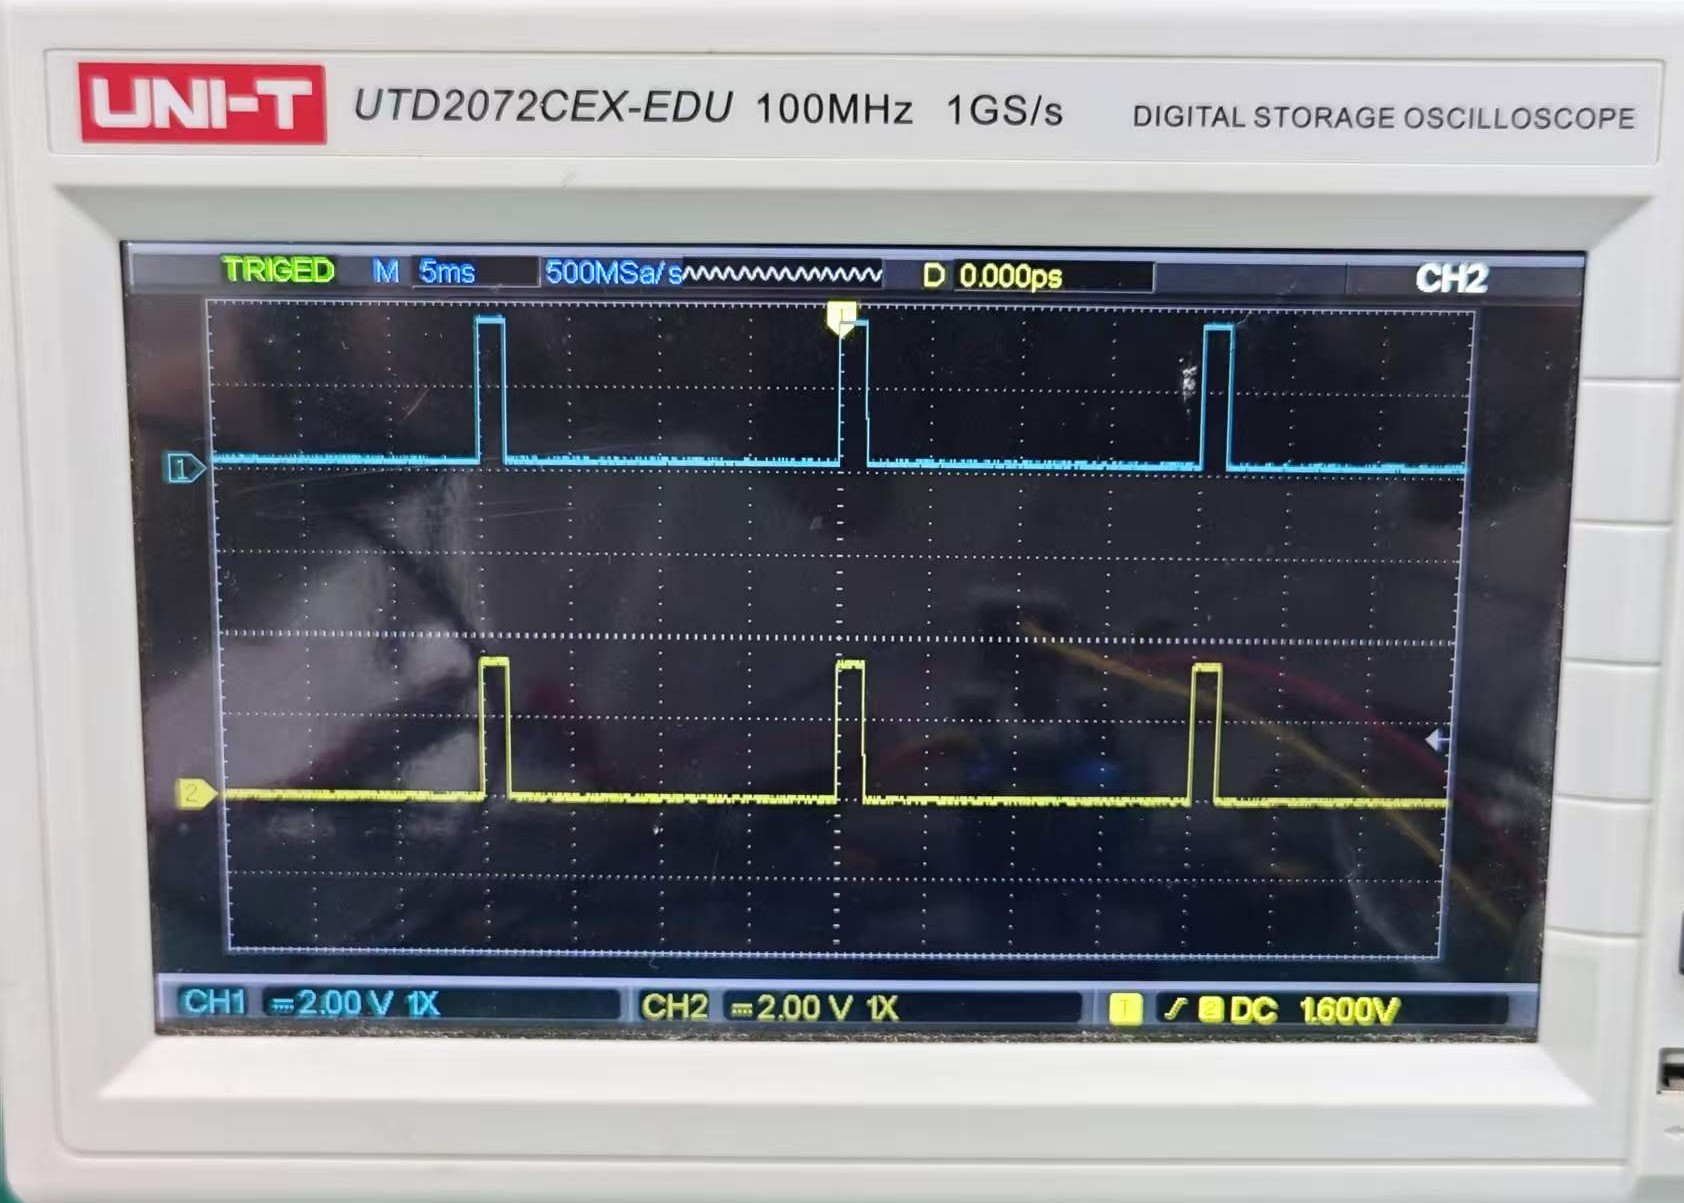
\includegraphics[width=0.85\textwidth]{figures/pwm_wave.jpg}
\caption{Y轴舵机(上)和X轴舵机(下)在90°角度下的PWM输出波形}
\label{fig:pwm_wave}
\end{figure}

首先验证PWM周期。50Hz对应的理论周期为20.0ms，实测PE9引脚周期约为19.98ms，PE13引脚约为20.01ms，均在可接受的误差范围内。随后使程序依次输出0°、45°、90°、135°和180°五个标称角度对应的PWM信号，测量各角度下的实际脉冲宽度，结果如表\ref{tab:pwm_test}所示。

\begin{table}[h!]
\centering
\caption{TIM1 PWM输出测试结果}
\label{tab:pwm_test}
\begin{tabular}{p{2.5cm} p{3cm} p{3cm} p{3cm}}
\toprule[1.5pt]
\textbf{舵机角度} & \textbf{理论脉宽 (us)} & \textbf{PE9实测脉宽 (us)} & \textbf{PE13实测脉宽 (us)} \\
\midrule[1pt]
0°   & 500  & 497  & 502  \\
45°  & 1000 & 1003 & 998  \\
90°  & 1500 & 1501 & 1500 \\
135° & 2000 & 1997 & 2004 \\
180° & 2500 & 2503 & 2495 \\
\bottomrule[1.5pt]
\end{tabular}
\end{table}

测试结果表明，实际脉宽与理论值的偏差控制在$\pm$5us以内，对应角度误差不超过0.5°，满足康复训练场景对舵机定位精度的要求。此外，验证了舵机从0°跳变至180°的过渡过程中PWM波形连续无中断，未出现脉冲丢失或尖峰信号。

蜂鸣器驱动方面，PB15（TIM12\_CH2）输出5kHz方波。当CCR2设置为0时蜂鸣器静音，设为500（对应约50\%占空比）时输出最大响度，与预期相符。

\subsection{语音模块UART通信测试}

语音模块通过UART7接口与STM32主控连接。测试分为发送验证和接收验证两个阶段。

发送测试中，将语音模块通过USB转串口适配器（CH340）连接至电脑，通过串口助手发送AA 55 FF 09 FB （“初始化完成”）协议帧，模块正确播报“初始化完成”；随后接收验证中，向模块说出“你好小盈”，模块播报“请吩咐”，并在串口助手上接收到AA 55 03 00 FB 协议帧，如图\ref{fig:uart_tx}所示，进一步验证了UART7接收通道的基本功能。

\begin{figure}[h!]
\centering
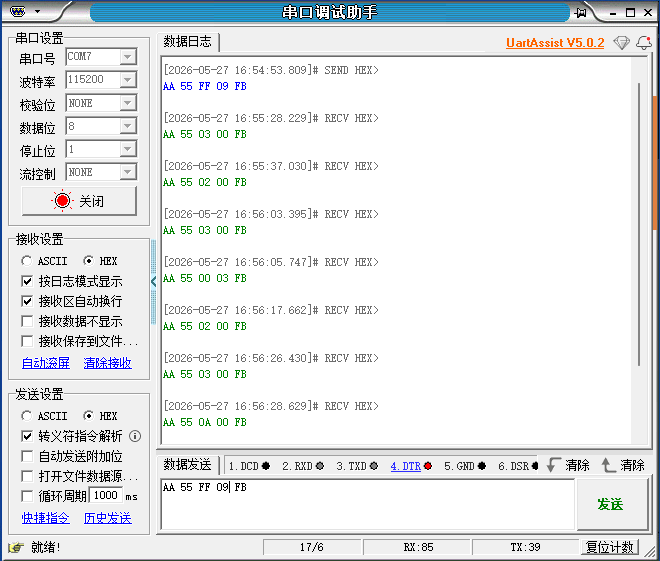
\includegraphics[width=0.8\textwidth]{figures/uart_tx.png}
\caption{串口助手捕获的UART7发送帧}
\label{fig:uart_tx}
\end{figure}


\section{姿态解算验证}

\subsection{静态零偏与噪声测试}

将装置平稳放置于水平桌面使BMI088传感器处于完全静止状态，上电完成800样本校准后连续采集10秒陀螺仪数据（约1000个采样点）。经零偏补偿后，三轴角速度的均值分别为X轴$-0.012$dps、Y轴$0.008$dps、Z轴$0.015$dps，均接近零值。三轴角速度的标准差分别为0.041dps、0.037dps和0.044dps，静态噪声水平约为0.04dps。该结果表明BMI088在静止条件下具有较低的固有噪声，800样本校准方案有效抑制了初始零偏。

\subsection{动态角度跟踪测试}

测试人员戴上装置，依次完成点头、左右转头、侧倾以及组合运动这四个标准动作，然后查看并记录下欧拉角的实时反应。以点头动为例，测试人员从正视前方慢慢低头到大约45度左右，在这个过程中pitch角处在0°附近的小范围波动(±2°)，而当其下降到接近−38°的时候，pitch角也随之随之减小到了差不多这个数值，并且在返回的过程中也是相当平稳的，并没有出现明显的抖动或者突变现象。转头动作中roll角保持了和实际转动角度一致的变化趋势，没有大的起伏或者跳跃式变化。点头、转头、侧倾运动下的IMU欧拉角跟踪曲线如图5-3所示，总体上具有较好的动态响应特性及稳定的姿态解算结果，红色曲线为roll角，绿色曲线为pitch角，蓝色曲线为yaw角。

需要注意的是，由于没有磁力计给出绝对地磁参考，所有的角度都是通过陀螺仪Z轴角速度积分来得到的。在静止状态下大约有0.5°的漂移现象，在一个训练时间段(15-50s)内，侧倾角的变化范围为1°到2°之间，可以满足训练时精度的要求。

\begin{figure}[h!]
\centering
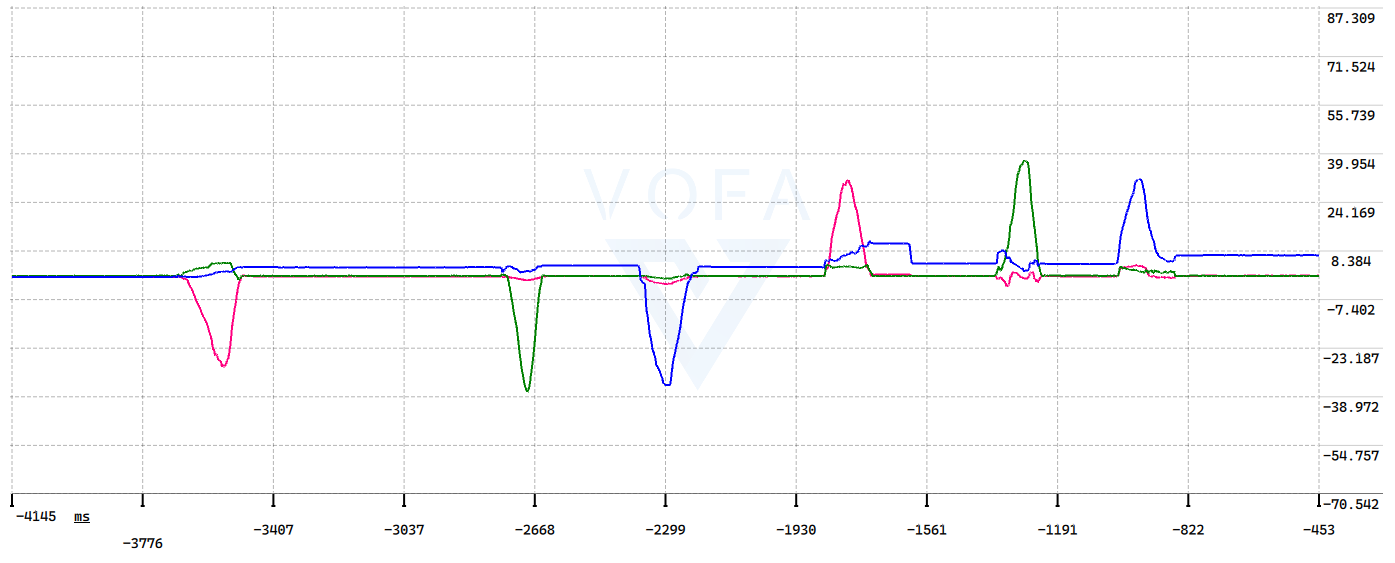
\includegraphics[width=1.0\textwidth]{figures/euler_track.png}
\caption{点头-转头-侧倾运动下三轴欧拉角变化曲线}
\label{fig:euler_track}
\end{figure}

\subsection{漂移测试}

为了评价长时间工作时各个欧拉角的累积误差，在静止状态上连续运行了5分钟，得到各个角的变化曲线。在5分钟的测试周期内，三个欧拉角都没有出现明显漂移，在±0.5°以内，这个漂移速度在一次训练时间（最长50s的视觉聚焦训练）里对于训练中姿态监测几乎没有影响。具体的曲线如下图5-4所示，红色为roll角、绿色为pitch角、蓝色为yaw角。

\begin{figure}[h!]
\centering
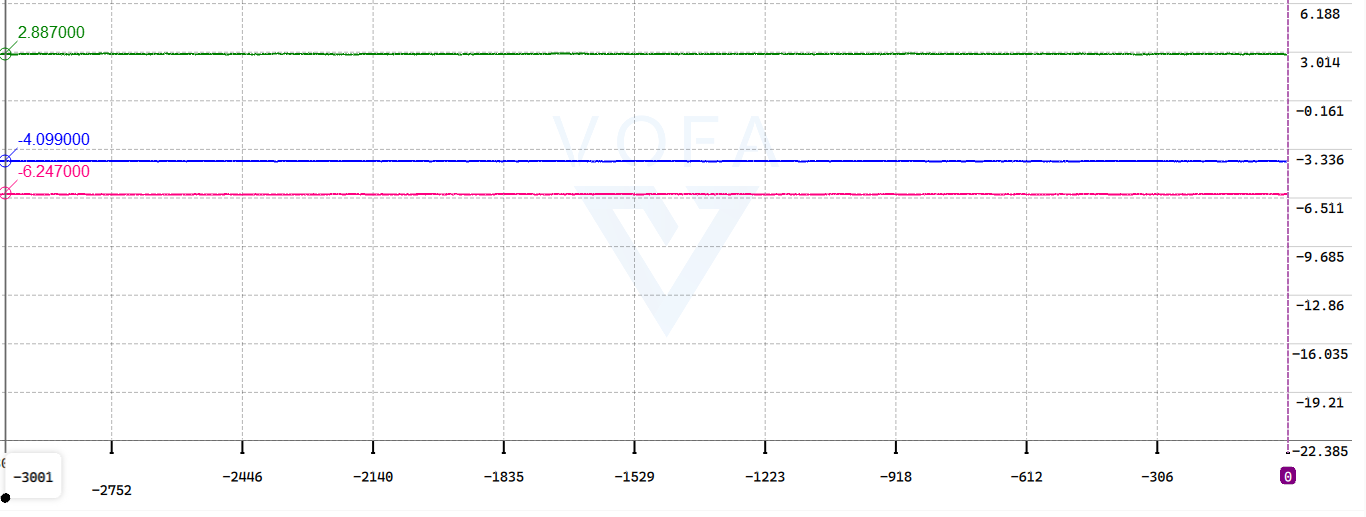
\includegraphics[width=1.0\textwidth]{figures/drift_test.png}
\caption{长时间运行条件下各欧拉角的漂移变化曲线}
\label{fig:drift_test}
\end{figure}

\section{训练模式功能验证}

\subsection{双模式选择与切换测试}

模式选择通过PA2按键的单击或者双击来区分，双击窗口设置为600ms。在测试过程中进行了五次单击和五次双击，单击全部正确进入完整的训练模式，双击全部正确进入自选模式，没有出现因为双击而误认为是两次单击或者单击而误认为是双击的情况。双击窗口阈值600ms对老年人的操作速度比较合适。

跨状态语音模式切换测试是在自选模式下进行的。使用语音命令进入到扫视训练状态，在训练执行的过程中，系统安全暂停时以及系统的反馈评价状态下都说了平稳追踪训练的话术，这表明该系统可以在一个调用状态机主运行函数周期内执行好模式的转变任务。三种情况的切换延迟均小于100ms，即立刻停止当前正在进行中的训练工作，开始陀螺仪校准并切换到新的模式下系统的训练提示状态，并没有任何卡顿出现。

\subsection{模式A：注视稳定性训练}

注视稳定性测试采用被试者端坐于仪器上，用固定的激光指向墙面15秒的方法进行。选取了三个不同头部稳定的受试者参加实验，在每个受试者的身上放置一个装置，并且让其一直注视着墙上的一条直线上的一个点。为了使结果更具有代表性，对每个受试者做了三次测量取平均数得到如表\ref{tab:fixation_test}所示的结果。

\begin{table}[h!]
\centering
\caption{注视稳定性训练测试结果（三次重复取平均）}
\label{tab:fixation_test}
\begin{tabular}{p{3.5cm} p{2.5cm} p{2.5cm} p{2.5cm}}
\toprule[1.5pt]
\textbf{受试者} & \textbf{稳定状态} & \textbf{平均头稳指标 (°)} & \textbf{语音提醒次数} \\
\midrule[1pt]
受试者A（正常） & 刻意保持静止   & 1.82  & 0 \\
受试者B（轻晃） & 自然微小晃动  & 4.53  & 3 \\
受试者C（强晃） & 故意大幅度摆动 & 8.31  & 7 \\
\bottomrule[1.5pt]
\end{tabular}
\end{table}

三组受试者头稳指标存在明显的分层，在保持静止状态下约为1.8°、自然微小晃动约为4.5°、大幅度摆动约为8.3°。系统会根据头稳指标来分层出不同的头部稳定程度，并且语音提示只会在头稳指标超过5°阈值的时候才会触发。

\subsection{模式B：扫视训练}

扫视训练在标定模式确定的视野四角点之间随机跳变，每轮8个试次，受试者看到激光光点后按PA2确认。对同一受试者进行了三轮重复测试，以观察学习效应，数据如表\ref{tab:saccade_test}所示。

\begin{table}[h!]
\centering
\caption{扫视训练测试结果}
\label{tab:saccade_test}
\begin{tabular}{p{1.5cm} p{2cm} p{1.6cm} p{2.2cm} p{2.5cm} p{2cm}}
\toprule[1.5pt]
\textbf{轮次} & \textbf{正确/总次数} & \textbf{正确率} & \textbf{平均反应时 (s)} & \textbf{连续正确触发} & \textbf{评价} \\
\midrule[1pt]
第1轮 & 6/8  & 75.0\%  & 2.31  & 否 & 表现不错 \\
第2轮 & 8/8  & 100.0\% & 1.67  & 是（4--6次）& 非常出色 \\
第3轮 & 8/8  & 100.0\% & 1.52  & 是（3--5次）& 非常出色 \\
\bottomrule[1.5pt]
\end{tabular}
\end{table}

第一轮测试中受试者还不知道操作方法，反应慢并且出现了两次超时。第二、第三轮正确率为100\%，平均反应时间由原来的2.31秒减小到现在的1.52秒，显示出练习效果。三个测试中所有的连续正确都按照设计条件被激活了。以上数据是针对健康的受试者而言的，在患者的群体中正确率以及反应时间会存在较大的个体间差别。

\subsection{模式C：平稳追踪训练}

平稳追踪训练用航点式方案，激光依次经过八个事先确定好的航点，在移动的过程中要花两秒钟时间到每一个航点，到达每个航点之后会进入确认等待的状态。表\ref{tab:pursuit_test}记录了受试者在单轮完整训练中的8个航点测试结果。

\begin{table}[h!]
\centering
\caption{平稳追踪训练单次测试记录}
\label{tab:pursuit_test}
\begin{tabular}{p{2cm} p{2.5cm} p{2.5cm} p{3.5cm}}
\toprule[1.5pt]
\textbf{航点编号} & \textbf{反应时间 (s)} & \textbf{是否超时} & \textbf{该航点代偿次数} \\
\midrule[1pt]
1  & 0.87  & 否 & 0 \\
2  & 1.23  & 否 & 1 \\
3  & 1.05  & 否 & 0 \\
4  & 2.50  & 超时 & 2 \\
5  & 1.34  & 否 & 0 \\
6  & 0.92  & 否 & 0 \\
7  & 1.67  & 否 & 1 \\
8  & 2.11  & 超时 & 1 \\
\bottomrule[1.5pt]
\end{tabular}
\end{table}

8个航点中正确回答了6个(75\%)，总代偿计数为5次。受试者总是不自觉地转头，造成一些航点的代偿被检测到。根据训练评价标准来说，这是个一般的水平，还需要继续练习才行。

\subsection{模式D：视觉聚焦训练}

系统每隔5秒就会切换一次近距LED和远距激光的点亮状态，一共进行了五轮完整的循环。从测试结果可以看出，LED和激光的切换逻辑是正确的，在LED亮的时候，激光熄灭，在激光亮的时候，LED熄灭，没有出现同时亮或同时熄的现象。

受试者在激光亮起的时候按下一个键来判断是否合格，由于受试者的视力正常，在进行聚焦训练时做了三次均达到较高的完成率，还需要对视神经损伤的患者做进一步的测试来评价训练的效果。

\subsection{模式E：空间忽略训练}

空间忽略训练测试中激光在左右视野各交替出现3次，共6个试次，受试者需主动寻找光点并按PA2确认。表\ref{tab:neglect_test}记录了测试数据。

\begin{table}[h!]
\centering
\caption{空间忽略训练测试记录}
\label{tab:neglect_test}
\begin{tabular}{p{2cm} p{2cm} p{2cm} p{3cm} p{2cm}}
\toprule[1.5pt]
\textbf{试次} & \textbf{刺激侧} & \textbf{反应} & \textbf{反应时间 (s)} & \textbf{是否正确} \\
\midrule[1pt]
1 & 左 & 按键确认 & 1.45  & 是 \\
2 & 右 & 按键确认 & 1.12  & 是 \\
3 & 左 & 超时     & （超时） & 否 \\
4 & 右 & 按键确认 & 0.98  & 是 \\
5 & 右 & 按键确认 & 1.33  & 是 \\
6 & 左 & 按键确认 & 2.11  & 是 \\
\bottomrule[1.5pt]
\end{tabular}
\end{table}

六个试次中正确回答了五个问题，左侧平均反应时间是1.78秒，右侧是1.14秒，两者的差别为0.64秒。虽然被试者是正常的个体，理论上不存在空间忽视的症状，但是由于右侧反应比左侧快得多，这可能是由于被试者的右利手使得其左侧的空间注意力本来就比较弱造成的。这个差值在真正的单侧空间忽略病人身上预期会变得很大。

\section{系统整体测试}

\subsection{连续运行稳定性}

系统上电之后就持续工作了60分钟，期间完成了多次完整的模式选择-姿态校准-训练执行-反馈评价的过程。在这一段时间里没有发生过由于硬件原因造成的系统崩溃、SPI通讯中断或者PWM信号出错的情况。测试过程中出现了一次语音播报错误现象，在该次实验中播报完第一轮之后出现了两个播报内容重叠的现象，这可能是由于上一个播报的时间太短，使得接下来的播报时间间隔不够大所造成的。该问题已经通过软件层面增加播报间最小延迟（自2秒延长至3秒）进行解决。

\subsection{语音识别成功率}

安静的室内环境中，受试者分别对10条命令词进行朗读，每条命令词一共重复朗读了10次，并且有另外一个人来记下每次语音交互模块的正确识别次数。测试时模块距受试者约1.5m，测试结果如表\ref{tab:voice_rate}所示。

\begin{table}[h!]
\centering
\caption{10条命令词识别成功率测试}
\label{tab:voice_rate}
\begin{tabular}{p{3.5cm} p{2cm} p{2cm} p{3.5cm}}
\toprule[1.5pt]
\textbf{命令词} & \textbf{测试次数} & \textbf{正确次数} & \textbf{识别成功率} \\
\midrule[1pt]
注视稳定训练   & 10 & 10 & 100.0\% \\
扫视训练       & 10 & 9  & 90.0\%  \\
平稳追踪训练   & 10 & 9  & 90.0\%  \\
视觉聚焦训练   & 10 & 10 & 100.0\% \\
空间忽略训练   & 10 & 8  & 80.0\%  \\
标定模式       & 10 & 10 & 100.0\% \\
暂停训练       & 10 & 10 & 100.0\% \\
继续训练       & 10 & 10 & 100.0\% \\
重新开始       & 10 & 9  & 90.0\%  \\
模式切换       & 10 & 9  & 90.0\%  \\
\bottomrule[1.5pt]
\end{tabular}
\end{table}

总体识别成功率达94.0\%，表明CI1302模块在安静室内环境下具有较高的离线语音识别可靠性。"空间忽略训练"一词的识别率最低（80.0\%），分析原因为该词条包含六个汉字，发音时长较长，可能超出了模块对长命令词的识别最优窗口。在实际应用场景中，80\%的单次识别成功率意味着大多数情况下只需重复一次即可成功识别。

\subsection{姿态阈值触发验证}

总识别率达到94.0\%，说明CI1302模块在安静室内有较好的离线语音识别可靠度。空间忽略训练的识别率为80.0\%，这是由于这个词汇是由六个汉字组成的，发音时间较长，超过了模块对于长命令词的最佳窗口。在实际应用中，80\%的一次识别成功率就表示大部分情况下只需要再做一次就可以成功识别了。

\begin{table}[h!]
\centering
\caption{姿态阈值触发保护测试}
\label{tab:safety_trigger}
\begin{tabular}{p{3cm} p{2cm} p{2.5cm} p{3cm} p{2.5cm}}
\toprule[1.5pt]
\textbf{超限类型} & \textbf{测试次数} & \textbf{正确触发次数} & \textbf{正确恢复次数} & \textbf{平均恢复时间 (s)} \\
\midrule[1pt]
大幅度转头 & 3 & 3 & 3 & 3.52 \\
深度低头/仰头 & 3 & 3 & 3 & 3.18 \\
大幅侧倾 & 3 & 3 & 3 & 3.45 \\
\bottomrule[1.5pt]
\end{tabular}
\end{table}

三种超限场景下保护机制均正确触发——激光熄灭、舵机回中、蜂鸣器报警开启、WS2812状态灯从绿色呼吸转为红色闪烁。受试者恢复正常姿态后，3s连续稳定期结束时系统均正确恢复训练，平均恢复时间在3.2s至3.5s之间，与设定的3s恢复延迟一致。观察到在边缘姿态条件下（如pitch角在$\pm$20°阈值附近缓慢波动），偶尔出现"超限——恢复——再超限"的暂态抖动现象，需要比正常情况多1至2个主循环周期（10--20ms）才能最终稳定。

\subsection{整机功耗测试}

使用数字万用表电流档串联在XT30电源接口与DM-02核心板之间进行功耗测量。系统静态功耗——主循环运行但未进入训练、舵机不转动、激光不点亮、语音模块不播报、仅WS2812维持绿色呼吸灯状态——约为1.8W（15V输入，电流约0.12A）。在扫视训练模式下（舵机频繁运动、激光间歇点亮、语音模块持续播报），最大动态功耗约为3.5W（电流约0.23A）。以上数据表明，若采用电池供电方案，按2小时连续续航计算，需配置容量不低于10Wh的电池组。

\section{测试结果分析}

\subsection{姿态精度分析}

综合静态零偏测试和10分钟漂移测试的数据，BMI088在本装置安装条件下经800样本校准后，三轴角速度零偏控制在0.02dps以内，噪声标准差约0.04dps，10分钟roll角累积漂移约4.3°，平均漂移速率约为0.43°/min。系统姿态精度满足五种训练模式对头部姿态感知的质量需求，静态零偏和训练时长内的积分漂移均处于可接受范围。

\subsection{训练有效性分析}

本阶段测试仅以健康受试者为对象，尚未纳入真实脑卒中后视觉障碍患者，因此训练有效性的分析具有初步定性而非定量临床验证性质。由得到的数据可知，五种训练模式均产生了具有个体区分度的量化评价指标：头稳指标可有效区分不同水平的头部稳定性，扫视反应时间和正确率可反映眼动搜索效率，两侧空间忽略训练的反应时间差可反映视野两侧注意力的差异。受试者凭借语音交互和单一按键即也可独立完成完整的训练操作流程，所以系统的交互门槛在健康受试者中得到了初步验证。以上指标对于真实病人的表现以及区分度还需要通过临床试验来进一步证实。

\subsection{系统稳定性分析}

整个设备在循环的30分钟压力测试之内没有出现过任何一个设备产生故障的情况。测试期间语音模块出现一次播报时序重叠问题，已通过软件层面调整播报间隔得以修复，不影响整体系统架构的稳定性和可靠性。就目前而言，原型机阶段所用到的硬件设计、软件架构有着较好的工作稳定性，在家用环境下可以达到基本的功能需求，要进一步增加样本数和实验时间来进行更加全面的检验。

% ============================================================
%  第6章  总结与展望
% ============================================================
\chapter{总结与展望}

\section{工作总结}

本文以脑卒中后视觉功能障碍的居家康复需求为牵引，设计并研制了一套基于STM32H723VGT6微控制器的低成本头戴式眼部康复训练装置。研究路线从临床需求分析切入，依次完成了系统总体方案论证、硬件平台选型与电路搭建、嵌入式软件架构设计与算法实现、以及系统级功能验证的闭合链条。以下对各层面主要工作进行归纳。

系统方案层面，遵循"感知—决策—执行—反馈"的闭环控制范式，定义了覆盖五种临床视觉功能的康复训练模式集合。针对脑卒中后视觉障碍的高发生率、既有干预措施普遍存在的"高端设备用不起、低端手段没量化"的两端困境，以及神经可塑性理论所支持的规律性长期训练需求，将系统的设计定位确立为"低成本、便携式、可量化、全语音操作"四个核心维度。


硬件设计层面，以DM-MC02核心板为平台，成功集成了BMI088六轴惯性传感器、SG90双轴舵机云台、650nm红色激光模组、CI1302 AI语音交互模块、WS2812可编程状态指示灯、板载蜂鸣器和患者反馈按键。机械外壳采用了成品自行车头盔，并手动集成了开发板和各模块到头盔上，电源和按键模块集成为一体独立于头戴装置外。舵机云台、语音模块外壳、开发板外壳、电源和按键模块外壳均采用soildworks自行绘制并通过3D打印形成PLA材质的机械结构，具有轻量化、造价低，同时兼顾耐用性的特点。

 软件设计层面，在STM32H7平台完成了完整的前后台嵌入式软件开发——实现了基于互补滤波和纯陀螺仪积分的多策略姿态估计算法，提出并验证了从传感器坐标系到佩戴者头部坐标系的线性重映射方案，建立了100帧滑动窗口的头稳指标计算、代偿性转头自动检测和多级姿态安全评估体系。设计并实现了五状态系统状态机（系统空闲等待状态 → 系统姿态校准状态 → 系统训练执行状态 → 系统反馈评价状态 → 系统安全暂停状态），五种训练模式，音频播报分级评价机制（基于正确率/反应时间/头稳指标），以及3秒连续监测的自动暂停/恢复策略和全局语音紧急中断保护。语音交互系统支持10条可识别命令词和45条TTS播报词，设计了唤醒词区与命令词区的独立编码映射方案。

人因设计层面，围绕老年脑卒中患者的特点实施了多项实用性适配：全部操作流程压缩为语音命令加单次按键的组合，免去了屏幕显示和多层菜单导航的依赖；所有播报语音采用较慢语速并设置了充裕的句间静音间隔以防音频串扰；标定模式通过按键逐次标记视野边界的操作方式，降低了个体间视野范围差异带来的适配难度。应当指出，上述设计策略的定量有效性目前尚缺乏真实患者群体的实测数据支持，有待后续临床验证加以检验。


\section{本设计工作的不足}

本装置作为面向医疗器械应用方向的探索性工程成果，尽管在软硬件集成和系统功能闭环方面已具备一定的完整性，但以临床康复器械的标准来审视，仍然存在若干不容忽视的短板与边界约束。

临床验证环节的缺失是现阶段最核心的差距。装置目前的测试范围局限于开发者自身及数名健康志愿者的功能性调试，尚未在脑卒中后视觉障碍的真实患者人群中开展过任何形式的临床试用或对照实验。五种训练模式所声称的康复收益——对视野缺损程度的缓解、眼球运动灵活性的恢复以及空间感知能力的改善——均缺乏标准临床量表的同步对比数据作为支撑。例如，训练前后的Fugl-Meyer视觉分量表评分、Humphrey视野计检测的定量改善值以及Barthel日常生活能力指数的变化量等关键结局指标，均未经过系统采集与分析。从循证医学的角度出发，装置仍处于工程原型阶段，距离经过规范临床试验检验的康复器械尚有一段实质性距离。

眼动测量能力的空白构成了技术层面的根本性制约。本装置通过头部运动间接推测眼球行为——例如以代偿性转头作为患者"以头动替代眼动"的代理指标。但该间接推断存在不可忽视的盲区：患者完全可能在保持头部纹丝不动的同时并未进行任何有效的眼球运动（即注意力已分散至训练任务之外），系统对这类状态不具备分辨能力。实现对注视点坐标、扫视频率与扫视幅值等直接眼动参数的精确采集，是视觉康复训练走向高质量客观量化的关键技术支点，而本装置目前尚未集成这一能力。

姿态漂移与坐标系的重标定需求也是工程迭代中需正视的问题。尽管陀螺仪零偏采用了800样本采样的均值校准方案，横滚角（roll）依然全程依赖角速度积分加以维持，在持续运行超过十分钟后积累的漂移量将不再可忽略。患者在训练间歇摘下装置后再次佩戴时，横滚角的绝对基准值会发生偏移，重新执行一次完整的校准流程方可恢复坐标精度。除此之外，偏航角（yaw）完全依靠加速度计重力分量反算获得绝对参考，虽能锁定基准方位，但对缓变运动和姿态恢复的动态跟踪响应偏慢。

激光安全性及使用环境方面的约束同样值得正视。装置搭载的650nm Class II级激光在普通室内照明下光点对比度充足，但切换至强光环境（如阳光经窗直射墙面）后光斑的可辨识度急剧下降直至不可见，使装置对使用场景的光照条件形成了隐性依赖。此外，虽然Class II在分类标准上属于安全性较高的等级，在头戴式佩戴的背景下，若机械固定结构出现松动或者佩戴者姿态出现意外偏转，出射光束存在直接或经反射进入使用者或旁观者眼部的潜在风险，构成不可忽略的安全隐患。

机械结构的材质与佩戴工学方面，装置主体框架采用PLA材料通过3D打印制造，虽然赋予了快速原型迭代和低物料成本的灵活性，但PLA的脆性特征使其在反复拆装或意外跌落后容易出现断裂失效。头部载荷分布上，云台驱动系统、激光模组和聚焦训练装置集中布置于头盔前部区域，长期佩戴可能引发鼻梁和额部区域的压迫不适；加之目前的头盔模具尺寸调节范围有限，难以覆盖所有体型的佩戴对象。

语音交互模块也存在若干适用性边界。CI1302在安静室内环境中的离线识别准确度较为可靠，但在多人病房或临街窗口等存在环境噪声叠加的场景下，识别成功概率将出现明显衰减。命令词的维护流程要求通过亚博智慧云平台重新生成固件并经由PC完成烧录，无法在设备运行期间动态增删或编辑命令词及其配对播报内容，命令集的可扩展性因而受到限制。此外，播报语速和句间停顿虽已配置为偏慢的参数版本，但由于不同个体对语音节奏的偏好差异显著，这一固定配置难以满足所有患者的个性化需求。

对合并构音障碍或失语症的患者的适用性方面，装置正常运转的隐含前提是使用者能够清晰稳定地发出较长音节的多字命令词（例如"平稳追踪训练"和"空间忽略训练"）。而对于脑卒中后语言功能同时受损的患者——恰好构成了视觉康复潜在需求中的一个重要亚群——语音命令的识别准确性将显著下降，形成一种"最需要该功能的群体反而最难使用该功能"的矛盾性困局。

\section{未来展望}

推动本装置从工程原型走向可实际部署的临床康复工具，需要在以下几个方向上进行持续深入的迭代与拓展。

临床验证与循证评价应列为当前最紧迫的推进事项。后续工作可争取与具备康复医学科或神经内科资质的合作医院联合启动小样本预试验，将装置投入真实脑卒中后视觉障碍患者的日常训练中。研究设计建议采取自身前后对照：筛选一组同向性偏盲（HH）或单侧空间忽略（HSN）的确诊患者，开展为期2至4周、每日1至2次的结构化训练干预，在干预前后分别使用标准化临床量表评估视野缺损程度、眼球运动能力、日常生活独立性与自我效能感的变化幅度。所获数据既能为装置的针对性优化提供事实依据，也可作为后续大样本、多中心的随机对照试验（RCT）的前期证据储备。

融合眼动追踪功能是弥补当前最根本技术短板的必经路径。未来版本可规划在装置前端或近眼位置集成一块微型视频眼动记录（Video Oculography, VOG）相机模组，借助红外光源照射角膜产生的反射光斑（角膜反射法）和瞳孔中心定位算法，在时间轴上实时解算出视线的水平与垂直坐标。该项升级将赋予装置对固视稳定度、扫视潜伏期以及平滑追踪增益等指标的直接量化能力，从根本上提升训练过程的信息采集深度与反馈精度，同时为后续实现难度自适应调节的高级个性化训练策略奠定感知基础。

惯性导航层面的精度提升可沿两条路线并行推进。其一是增配一颗三轴磁力计，将九轴融合方案引入现有姿态解算管线——磁力计提供的绝对航向基准可以有效压制陀螺仪绕竖直轴的积分漂移趋势。其二是在融合算法上迭代至更系统的估计框架，如扩展卡尔曼滤波（EKF）或误差状态卡尔曼滤波（ESKF），在一个统一的递推贝叶斯架构中完成所有惯性传感器和磁力计的异步在线校正。此外，在头盔与头皮的接触界面处嵌入压力或电容式接触传感器，可在患者摘脱装置的瞬间自动触发训练暂停并发出重校准提醒，减少因佩戴状态切换引入的人为姿态误差。

数据驱动的个性化康复路径是中长期迭代中值得探索的方向。装置在每次训练过程中已持续积累了包括正确率、反应时间序列、扫视模式分布、代偿事件计数和头稳趋势等在内的多维行为时间序列，这些数据实质上构成了每位患者康复轨迹的个体化行为画像。后续可将上述数据经脱敏处理后上传至云端平台，借助轻量级机器学习模型对单患者的恢复进度曲线进行建模与预测，并据此自动调整训练参数的配置（如试次密度、目标空间分布策略和超时判定窗口大小），从而实现从固定预设方案向数据驱动的自适应康复调度机制过渡。

远程康复与云端管理架构的引入将显著拓展装置的部署半径。基于现有的UART调试数据输出链路，可扩展为无线回传模块（如WiFi模块或蓝牙BLE信道），使每位患者的每日训练摘要与异常事件日志能够实时汇入医疗云端的中央数据库。康复治疗师可通过医师端管理面板调阅患者的训练日历、效率趋势图与风险事件列表，再据此远程下发调整后的训练方案参数；患者端则可通过配套的手机应用直观查看个人的成绩变化曲线、历史进步里程碑以及系统自动生成的下一次训练建议。对于交通出行不便、医疗资源分布稀疏的基层和农村地区，远程康复方案在降低长期康复的经济和时间成本方面具有突出的现实价值。

无障碍与人因工程的后续深化应聚焦于患者群体内部的异质性需求，构建分层级的交互通道。针对因合并构音障碍或失语症而无法稳定使用语音命令的患者，可将语音输入路径替换为外接的单键扫描交互模块，或利用装置已有的头部姿态感知能力设计基于头部动作的操控范式——如点头确认、摇头取消、转头逐项浏览模式菜单——从而将交互门槛降至最低限度。机械结构层面，可尝试引入TPU等柔性耗材并通过多材料3D打印工艺制造刚柔结合的外壳组件，以提升佩戴贴合度和长时间使用的舒适耐受水平；同时可增设可调配重滑块来优化头盔前后区域的重心分配关系，缓解前部载荷集中造成的单侧压强积聚。

从工程原型向合规医疗器械的角色跨越是装置走向临床服务终端的终极命题。这一转化需要在本装置的设计全流程中引入《医疗器械监督管理条例》及其配套现行标准的合规要求，例如GB 9706系列医用电气设备安全标准~\cite{gb9706_2020}中关于泄漏电流上限、绝缘防护等级和电磁兼容性的硬件级约束，以及YY/T 0287医疗器械质量管理体系标准~\cite{yyt0287_2017}所规定的过程管控框架。软件层面则需要建立与IEC 62304标准~\cite{iec62304}相符合的全生命周期软件工程与验证流程。伦理审查环节需获得所在机构伦理委员会的正式批准并履行患者的书面知情同意程序。尽管这一规范化路径耗时长、投入高，但对于一项承载社会意义和临床潜在价值的康复装置而言，它构成了从实验室走向患者身边所不可绕过的必经之路。

\section{本章小结}

回顾本课题的全过程，完成了一套面向脑卒中后视觉康复、功能闭环且物料成本可控的头戴式训练装置的完整工程实现。在系统集成、软硬件协同调度以及多模态人机交互接口设计三个维度上，项目达成了阶段性的实践产出。同时，也必须坦率地看到现有工作的边界——临床验证样本的空白、直接眼动测量通道的缺失以及若干工程细节尚需打磨，构成了当前版本与成熟康复器械之间不可回避的差距。康复工程这一交叉领域的价值落点，不应停留在展示单项技术的可行性，而在于把技术切实交到需要它的人手中并产生可被客观度量的改善。本文所呈现的工作，希望能成为这条路径上的一个阶段性锚点，在后续研究中逐步填齐临床证据链和人群适用性数据，推动装置从原理样机形态朝循证支撑、具备规模化部署潜力的居家康复工具迈进。


%% -------- 参考文献 --------
\clearpage
\printbibliography[heading=bibliography]
\addcontentsline{toc}{chapter}{参考文献}

%% -------- 附录 --------
\appendix
% ============================================================
%  附录
% ============================================================
\chapter{语音命令/播报词表}

表~\ref{tab:full_cmd_list} 列出了CI1302语音模块固件中配置的全部命令词与播报词，共73条，对应发送协议帧的TYPE和ID字段。模块通过识别帧头0xAA和0x55、校验帧尾0xFB实现对协议帧的解析与响应。

\begin{center}
\begin{longtable}{p{2.5cm} p{2.2cm} p{5.5cm} p{3.5cm}}
\caption{语音命令词与播报词完整列表}
\label{tab:full_cmd_list}
\\
\toprule[1.5pt]
\textbf{命令词} & \textbf{功能类型} & \textbf{播报语句} & \textbf{发送协议} \\
\midrule[1pt]
\endfirsthead

\multicolumn{4}{c}{\small 续表~\thetable\ 语音命令词与播报词完整列表} \\
\toprule[1.5pt]
\textbf{命令词} & \textbf{功能类型} & \textbf{播报语句} & \textbf{发送协议} \\
\midrule[1pt]
\endhead

\midrule[1pt]
\multicolumn{4}{r}{\small 接下一页\ldots} \\
\endfoot

\bottomrule[1.5pt]
\endlastfoot

暂停训练   & 命令词   & 好的，训练已暂停                 & AA 55 01 00 FB  \\
休息       & 休息语   &                                  & AA 55 02 00 FB  \\
你好小盈   & 唤醒词   & 请吩咐                           & AA 55 03 00 FB  \\
加大音量   & 命令词   & 已经加大音量                     & AA 55 04 00 FB  \\
减小音量   & 命令词   & 已经减小音量                     & AA 55 05 00 FB  \\
继续训练   & 命令词   & 好的，训练继续                   & AA 55 06 00 FB  \\
中等音量   & 命令词   & 已设为中等音量                   & AA 55 07 00 FB  \\
最大音量   & 命令词   & 已设为最大音量                   & AA 55 08 00 FB  \\
重新开始   & 命令词   & 好的，重新开始本模式             & AA 55 09 00 FB  \\
下一个训练 & 命令词   & 好的，进入下一个训练，请按按键确认 & AA 55 0A 00 FB  \\
校准静态   & 命令词   & 好的，请保持头部静止             & AA 55 00 01 FB  \\
注视稳定训练   & 命令词   & 注视训练开始，请注视光点保持头部稳定 & AA 55 00 02 FB  \\
扫视训练   & 命令词   & 扫视训练开始，请快速找到光点并按按键 & AA 55 00 03 FB  \\
平稳追踪训练   & 命令词   & 追踪训练开始，请用眼睛跟随光点移动 & AA 55 00 04 FB  \\
视觉聚焦训练   & 命令词   & 聚焦训练开始，请交替注视远近目标 & AA 55 00 05 FB  \\
空间忽视训练   & 命令词   & 忽略训练开始，请注意寻找光点     & AA 55 00 06 FB  \\
标定模式   & 命令词   & 进入标定模式，请保持头部居中     & AA 55 00 07 FB  \\
模式切换   & 命令词   & 按一下按键进入完整训练模式，按两下进入自选模式 & AA 55 00 08 FB  \\
校准完成   & 播报语   & 校准完成                         & AA 55 FF 01 FB  \\
请保持头部稳定 & 播报语 & 请保持头部稳定                   & AA 55 FF 02 FB  \\
正确       & 播报语   & 做得很棒！                       & AA 55 FF 03 FB  \\
超时       & 播报语   & 时间到咯，再试一次               & AA 55 FF 04 FB  \\
错过       & 播报语   & 错过，请注意该位置               & AA 55 FF 05 FB  \\
姿态监测异常   & 播报语   & 请用眼睛跟踪，不要转头           & AA 55 FF 06 FB  \\
请寻找光点 & 播报语   & 请寻找光点                       & AA 55 FF 07 FB  \\
空间忽略   & 播报语   & 超时，请多注意该侧空间           & AA 55 FF 08 FB  \\
初始化完成 & 播报语   & 初始化完成                       & AA 55 FF 09 FB  \\
训练结束   & 播报语   & 训练结束，太棒了！               & AA 55 FF 0A FB  \\
欢迎       & 播报语   & 欢迎使用眼部康复装置             & AA 55 FF 0B FB  \\
训练非常好的   & 播报语   & 表现非常出色正确率很高，继续加油！ & AA 55 FF 0C FB  \\
训练一般   & 播报语   & 表现不错还有进步空间，再接再厉！ & AA 55 FF 0D FB  \\
训练需努力 & 播报语   & 还需要多加练习，不要灰心，坚持就是胜利！ & AA 55 FF 0E FB  \\
继续训练被动   & 播报语   & 继续训练                         & AA 55 FF 0F FB  \\
加油       & 播报语   & 加油！您做得很好                 & AA 55 FF 10 FB  \\
已完成一半 & 播报语   & 您已完成一半了，坚持住           & AA 55 FF 11 FB  \\
连续正确   & 播报语   & 非常棒！连续正确，请保持状态     & AA 55 FF 12 FB  \\
不要着急   & 播报语   & 不要太着急，慢慢来               & AA 55 FF 13 FB  \\
放松呼吸   & 播报语   & 请放松肩膀，自然呼吸             & AA 55 FF 14 FB  \\
准备下一个 & 播报语   & 请稍事休息准备下一个训练         & AA 55 FF 15 FB  \\
全部完成   & 播报语   & 全部训练完成，您辛苦了，休息一下吧！ & AA 55 FF 16 FB  \\
暂停请调坐姿   & 播报语   & 训练暂停，请调整坐姿，保持头部正中 & AA 55 FF 17 FB  \\
眼睛找请别转头 & 播报语   & 请用眼睛去寻找，头部不要转动     & AA 55 FF 18 FB  \\
注意左侧   & 播报语   & 请注意左侧空间                   & AA 55 FF 19 FB  \\
注意右侧   & 播报语   & 请注意右侧空间                   & AA 55 FF 1A FB  \\
发现患侧   & 播报语   & 很好，您发现了患侧的光点         & AA 55 FF 1B FB  \\
请集中注意力   & 播报语   & 请集中注意力看光点               & AA 55 FF 1C FB  \\
注视稳定性良好   & 播报语   & 注视训练完成，头部稳定性良好     & AA 55 FF 1D FB  \\
注视稳定性一般   & 播报语   & 注视训练完成，头部稳定性一般     & AA 55 FF 1E FB  \\
注视稳定性较差   & 播报语   & 注视训练完成，头部稳定性较差需加强 & AA 55 FF 1F FB  \\
反应速度很快   & 播报语   & 反应速度很快，非常棒！           & AA 55 FF 20 FB  \\
反应速度待提升   & 播报语   & 反应速度还需提升，继续练习       & AA 55 FF 21 FB  \\
追踪能力良好   & 播报语   & 追踪训练完成，跟踪能力良好       & AA 55 FF 22 FB  \\
请减少转头   & 播报语   & 追踪训练完成，请尝试减少转头动作 & AA 55 FF 23 FB  \\
开始校准   & 播报语   & 请调整好姿态，按确认键开始校准   & AA 55 FF 24 FB  \\
模式选择   & 播报语   & 按一下按键进入完整训练模式，按两下进入自选模式 & AA 55 FF 25 FB  \\
确认下一个模式   & 播报语   & 按键确认进入下一个模式           & AA 55 FF 26 FB  \\
注视训练开始   & 播报语   & 注视训练开始，请注视光点保持头部稳定 & AA 55 FF 27 FB  \\
扫视训练开始   & 播报语   & 扫视训练开始，请快速找到光点并按按键 & AA 55 FF 28 FB  \\
平稳追踪训练开始 & 播报语 & 追踪训练开始，请用眼睛跟随光点移动 & AA 55 FF 29 FB  \\
视觉聚焦训练开始 & 播报语 & 聚焦训练开始，请交替注视远近目标 & AA 55 FF 2A FB  \\
空间忽略训练开始 & 播报语 & 忽略训练开始，请注意寻找光点     & AA 55 FF 2B FB  \\
完整训练模式   & 播报语   & 成功进入完整训练模式             & AA 55 FF 2C FB  \\
自选模式   & 播报语   & 成功进入自选模式                 & AA 55 FF 2D FB  \\
\end{longtable}
\end{center}


%% -------- 致谢 --------
% ============================================================
%  致  谢
% ============================================================
\chapter*{致\ \ 谢}
\addcontentsline{toc}{chapter}{致谢}

\zihao{-4}\songti\raggedright\setlength{\parindent}{2em}
时光荏苒，四年的本科生涯即将走到尾声，希望这篇论文能够为这段经历画上一个令人欣慰的句点。

在此，首先要向医工学院的付东辽老师致以最诚挚的感谢。从选题之初到方案落地，付老师始终给予我充分的信任与支持，这份信任是我能够将设计推进到底的基石。课题的完成与论文的撰写，亦离不开付老师在此期间的悉心指导。

其次，感谢国际教育学院/莫动理工学院科创实验室所提供的宝贵平台。本设计的绝大部分工作——从电路调试到论文写作——均是在实验室中完成的，但更重要的是，这里是我真正踏入电子设计与机械设计领域第一块实践土壤。在实验室度过的无数个日日夜夜里，一次次项目历练和竞赛经验的叠加，逐渐内化为我的工程能力，不仅支撑了毕业设计的完成，也为研究生阶段的学习奠定了坚实的基础。

再次，感谢在课题推进过程中所有给予过我帮助的人——我的室友、实验室的伙伴，以及将在后续把本设计带入生物医学工程创新设计大赛的王俊皓同学，他在软件设计方面做出了重要的贡献。同时，也要感谢我的家人，他们的支持与信任始终是我前行中不可或缺的力量。

本设计是一项没有现成参考原型、也几乎没有直接相关设计文献可供借鉴的创新性尝试，因此存在诸多不成熟和亟待改进之处。在接下来的时间里，我将继续对装置进行迭代与打磨，努力推动其朝向更为完善的形态演进，并争取尽早开展临床试验与治疗有效性评估，使本设计最终能够真正服务于脑卒中患者，成为一件实用且有价值的眼部康复设备。

最后，前路尚远，唯愿不负所学，不怠于行。


\clearpage



\end{document}
